\documentclass{report}

\usepackage[utf8]{inputenc}
\usepackage[T1]{fontenc}
\usepackage[francais]{babel}
\usepackage[textwidth = 400pt]{geometry}
\usepackage{url}
\usepackage{graphicx}
\usepackage{float}
\usepackage{longtable}
\usepackage{csvsimple}
\usepackage[table]{xcolor}
\usepackage{color}
\usepackage{lastpage}
\usepackage{fancyhdr}
\usepackage{appendix}
\usepackage{hyperref}



\begin{document}


\title {Projet de réalisation d'une IHM : OptiFret Lyon \\ Conception de l'IHM}
\author{Dragibus}
\maketitle


\newpage
~~\\
\textbf{Equipe Dragibus} : Hexanôme H4104 \\
Patrizia Peller\\
Mathis Paul\\
Sylvain Abadie\\
Quentin Coursodon\\
Pierre Turpin\\
Jean Marie Comets\\
Julien Rollet\\

~~\\
\textbf{Responsable Qualité} : Patrizia Peller\\
~~\\
\textbf{Gestion de Projet} : Julien Rollet\\


\tableofcontents


%-------------------DTU-------------------------%

\chapter{Description des Tâches de l'Utilisateur}

\paragraph{}
Pour cette première partie de la conception d'OptiFret, nous avons séparé l'équipe en deux groupes de travail :\\
Equipe A : Q Coursodon, M Paul, P Peller \\
Equipe B : P Turpin, S Abadie, JM Comets\\

L'Equipe A a travaillé sur : DDF \\

L'Equipe B a travaillé sur : MU / DPU / GPU \\

L’ensemble de l’équipe a travaillé sur : TTU / DF, DTU / DF, SPU \\


Cette première partie détaille essentiellement les activités de l'entreprise concernée et des utilisateurs ayant trait à l'application en développement.

\section{Description des Domaines Fonctionnels}

\begin{tabular}{|c|c|l|}
\hline
D.1 & Administration des Systèmes informatiques& D.1.1 Maintenance\\
&&																							 D.1.2 Gestion utilisateurs\\
\hline
D.2 & Gestion des Ressources Humaines & D.2.1 Recrutement\\
&&																			D.2.2 Gestion du personnel\\
\hline
D.3 & Comptabilité & D.3.1 Gestion couts internes\\
&&									 D.3.2 Gestion salaires\\
&&									D3.3 Gestion factures clients\\
\hline
D.4 & Gestion des relations clientèles & D.4.1 Gestion SAV\\
&&																			D.4.2 Gestion contrats\\
\hline
D.5 &  Gestion des livraisons & D.5.1 Gestion des demandes de livraison\\
&&															D.5.2 Préparation et supervision des livraisons\\
&&															D.5.3 Réalisation des livraisons\\
\hline
\end{tabular}
~~\\
~~\\
D.1.1 Maintenance corrective et préventive permettant le bon fonctionnement du SI.\\
D.1.2 Création des utlisateurs, type d’utilisateur, gestion des droits.\\
~~\\
D.2.1 Ensemble des actions et démarche pour trouver sélectionner des candidats.\\
D.2.2 Gestion des congés, des abscences, formation continue.\\
~~\\
D.3.1 Gestion comptable de l’entreprise.\\
D.3.2 Gestion de la rémunération des employés.\\
D.3.3 Suivi des paiements par les clients.\\
~~\\
D.4.1 Prise en compte des plaintes des utilisateurs.\\
D.4.2 Démarchage des clients et négociation de contracts.\\
~~\\
D.5.1  Enregistrement des demandes de livraison, mise en relation du client et de l’entreprise de transport.\\
D.5.2 Génération des feuilles de routes, modification des feuilles de routes, suivi de l’états des livraisons en cours, des livreurs.\\
D.5.3 Transport des colis entre l'entrepôt du fournisseur et le client.\\

\paragraph{}

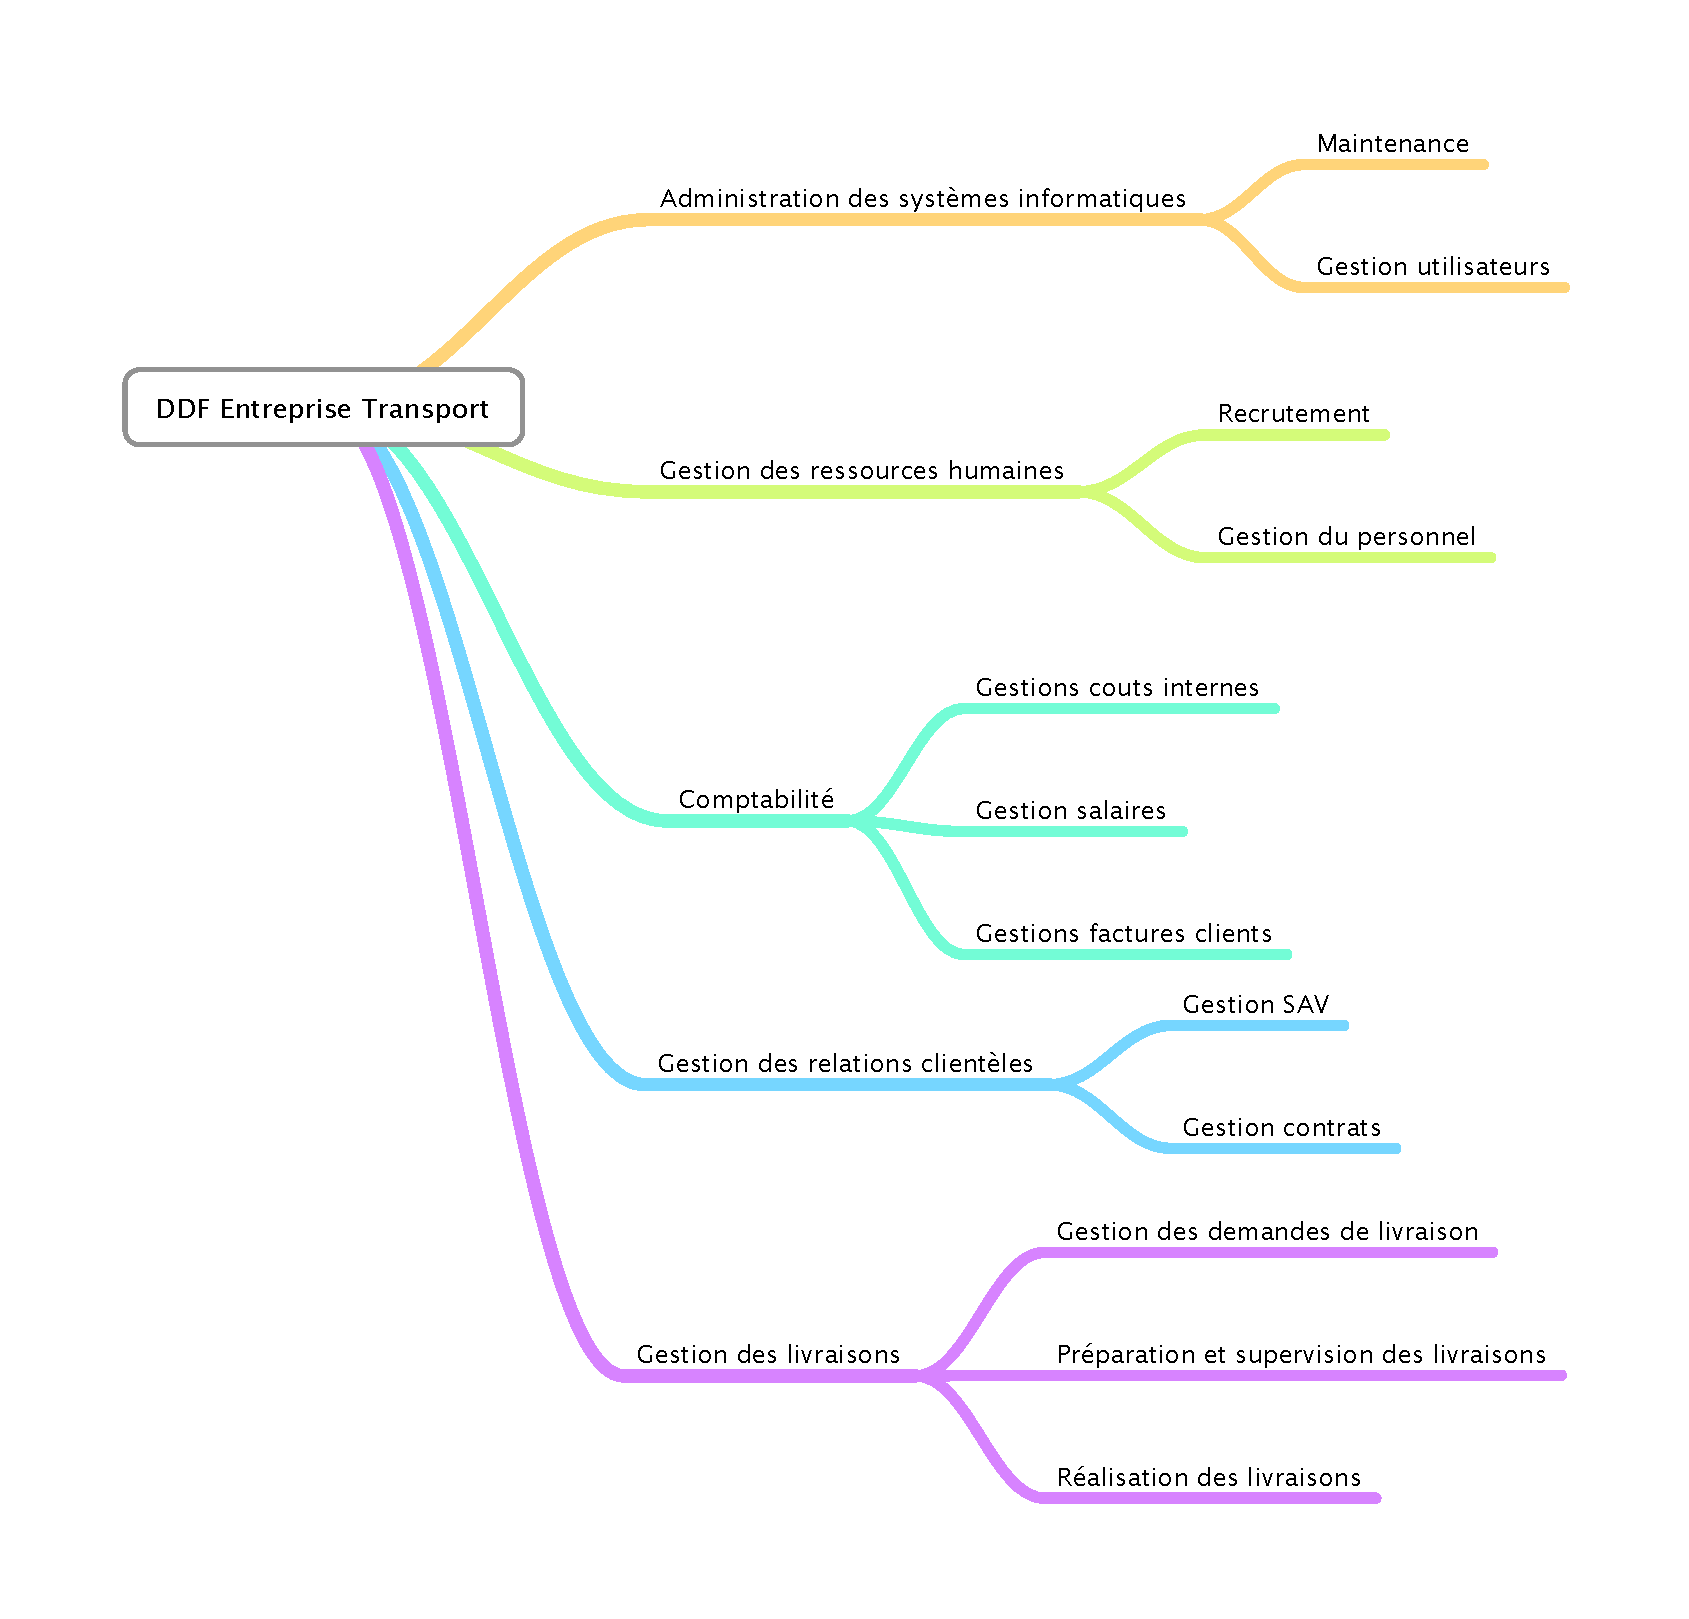
\includegraphics[scale = 0.4]{images/DDF.pdf}


\section{Modèle des Utilisateurs}

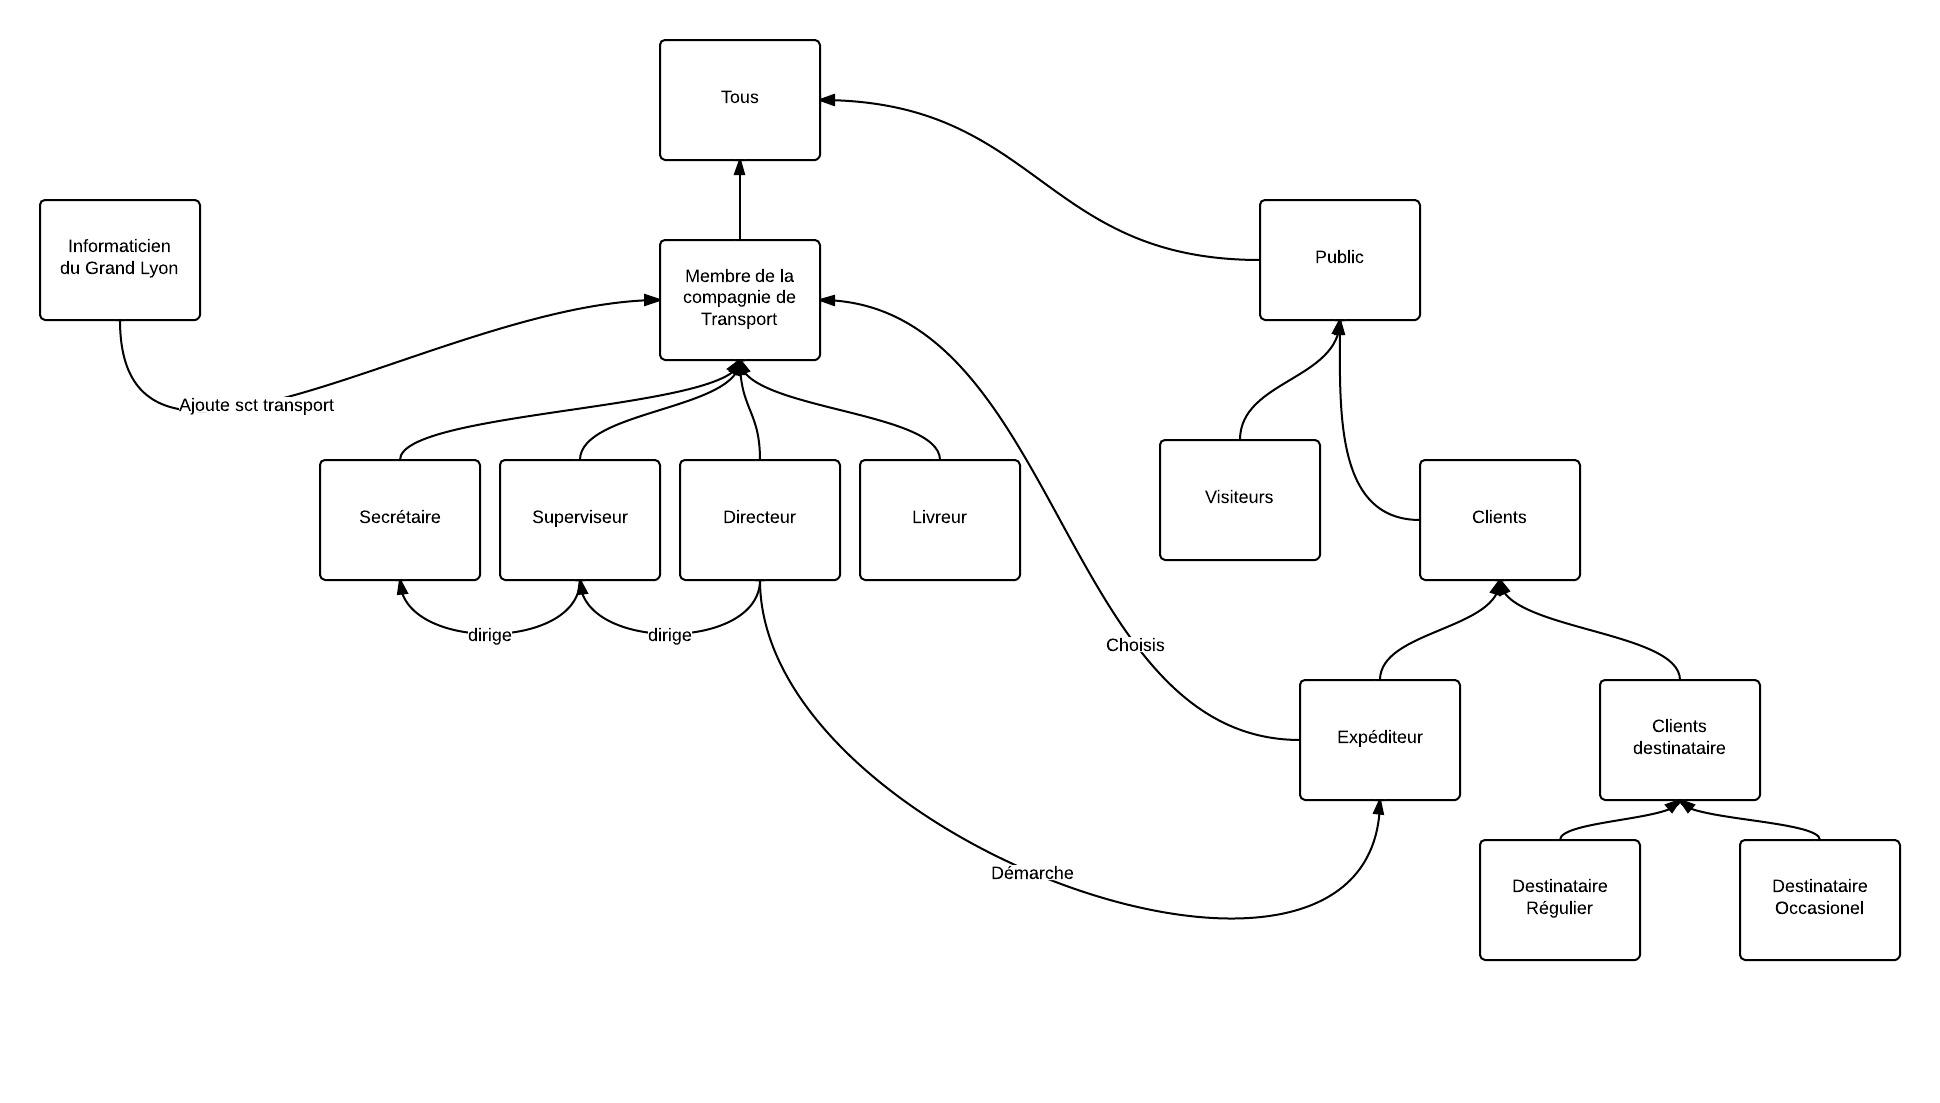
\includegraphics[scale = 0.3, angle=90]{images/MU.jpeg}

\section{Graphe d'héritage des Profils Utilisateurs}

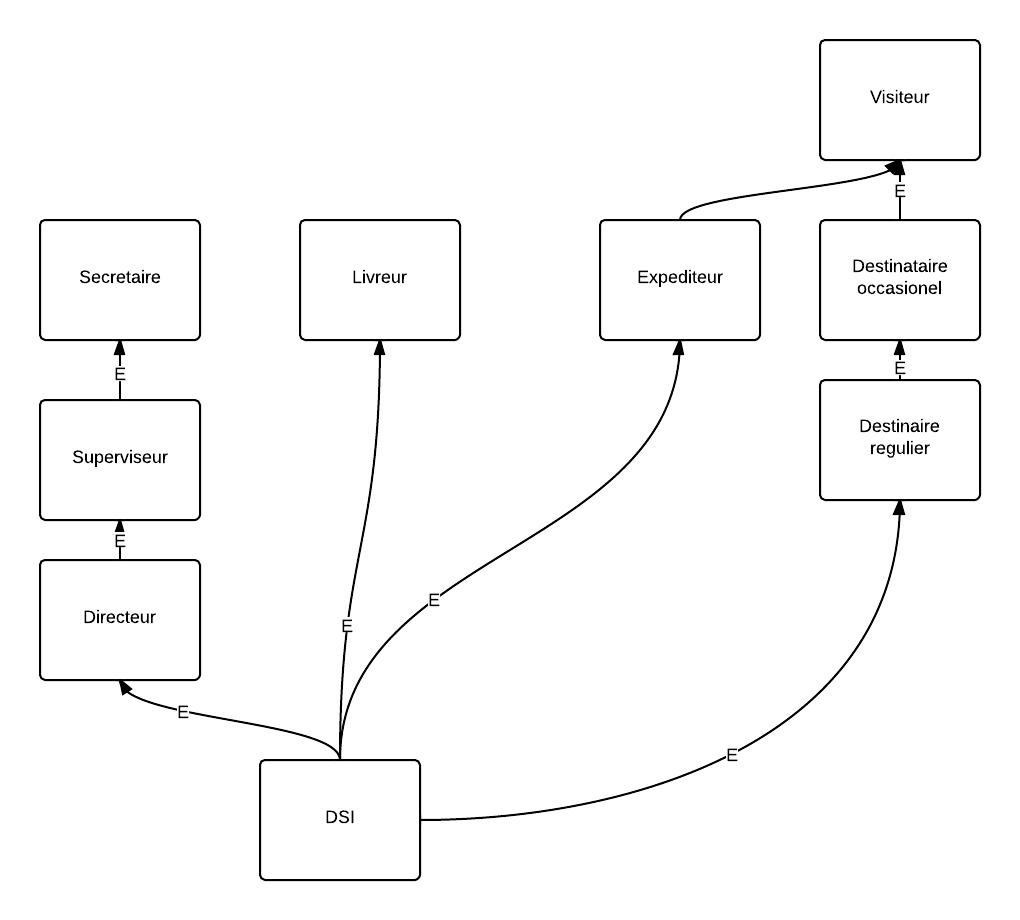
\includegraphics[scale = 0.25]{images/GPU.jpeg}

\section{Description des Profils Utilisateurs}

\begin{itemize}

\item{Directeur:} Directeur d’une entreprise de transport. Gère son entreprise en démarchant des clients ayant besoin d’expédier des marchandises (ex : amazon, fnac ...). Il dirige les superviseurs et les secrétaires et peut potentiellement les remplacer dans leurs tâches.\\ 

\item{\hypertarget{labDPULiv}{Livreur} :} CFP (contrat de formation professionnelle) de livreur, doit être détenteur d’un permis B (conduite de véhicule léger allant jusqu’à 3,5 tonnes). Il se doit d’être ponctuel et actif. Il doit également connaître la zone géographique dans laquelle il livre.  Doit se familiariser avec l’interface de livraison (feuille de route, horaires) et le système de signalisation de changement (info trafic, client non livré/absent).\\

\item{\hypertarget{labDPUSec}{Secrétaire} :} Possède une formation de secrétariat. Doit savoir utiliser l’interface de suivi de livraison des clients dans le cas où ceux-ci ne sont pas à l’aise avec INTERNET. Contact également les clients dont leur livraison prévues n’a pas pu être effectué soit à cause de l’absence du dit client, soit à cause d’un autre problème.\\

\item{\hypertarget{labDPUSup}{Superviseur} :} Il doit avoir un diplôme d’ingénieur ou de management, son poste ayant de lourdes responsabilités. Il appartient à la société de livraison et contrôle en temps réel le déroulement des livraisons. Il possède les droits pour modifier interractivement les feuilles de route afin d’optimiser les temps ou de gérer des évènements imprévisibles (incidents … ).\\

\item{Visiteur :} Utilisateur découvrant l’interface Web sans pour autant être inscrit ou connecté au système.\\

\item{Expéditeur :} Employé de magasin, il reçoit des commandes pour ses produits et souhaite effectuer des livraisons dans les délais imposés. Il doit savoir utiliser l’interface Web pour définir les livraisons (info, destinataire, livreur). Ils peuvent contacter une secrétaire de l’entreprise de transport pour gérer le suivi de leur livraison dans le cas où ils ne sont pas à l’aise avec l’interface Web.\\

\item{Destinataire Occasionnel :} Particulier ou professionnel, il veut recevoir sa commande à l’horaire qui l’arrange. Il se connecte via des identifiants qui lui sont communiqués par l’expéditeur. Il peut demander une inscription s’il s’avère utile d’avoir une démarche plus rapide. Il peut savoir utiliser l’interface Web pour visualiser et modifier les livraisons mais peut demander à la secrétaire de la société de livraison de le faire à sa place. Signe un reçu sur réception du colis et peut éventuellement faire une réclamation dans le cas où le colis est dans un mauvais état.\\


\item{Destinataire régulier :} Le destinataire régulier se distingue du destinataire occasionnel par le fait qu’il est inscrit avec un nom d’utilisateur et un mot de passe évitant ainsi de donner à nouveau son adresse.\\

\item{Informaticien du Grand Lyon :} Groupe administrant et maintenant le système. Responsable de l’ensemble des composants matériels (postes de travail, serveurs, équipements de réseau, systèmes de stockage, de sauvegarde) et logiciels du système informatique.\\

\end{itemize}

\section{Tableau des Tables Utilisateurs par Domaine Fonctionnel}

\begin{tabular}{|p{5cm}|p{3cm}|p{3cm}|p{3cm}|}
\hline
&D1) Gestion des Livraisons & D2) Gestion des relations Clientèles & D3) Admin. SI\\
\hline
U1) Visiteur&&\textit{T.1.2}&\\
\hline
U2) Destinataire occasionnel&&T.2.2&\\
\hline
U3) Destinataire régulier &&\textbf{T.3.2}&\\
\hline
U4) Expéditeur&&\textbf{T.4.2}&\\
\hline
U5) Livreur&\textbf{T.5.1}&&\\
\hline
U6) Secrétaire&T.6.1&T.6.2&\\
\hline
U7) Superviseur&\textbf{T.7.1}&T.7.2&\\
\hline
U8) Directeur&\textit{T.8.1}&T.8.2&\\
\hline
U9) Informaticien du Grand Lyon&\textit{T.9.1}&\textit{T.9.2}&\textbf{T.9.3}\\
\hline
\end{tabular}

\section{Description des Tâches Utilisateurs par Domaine Fonctionnel}

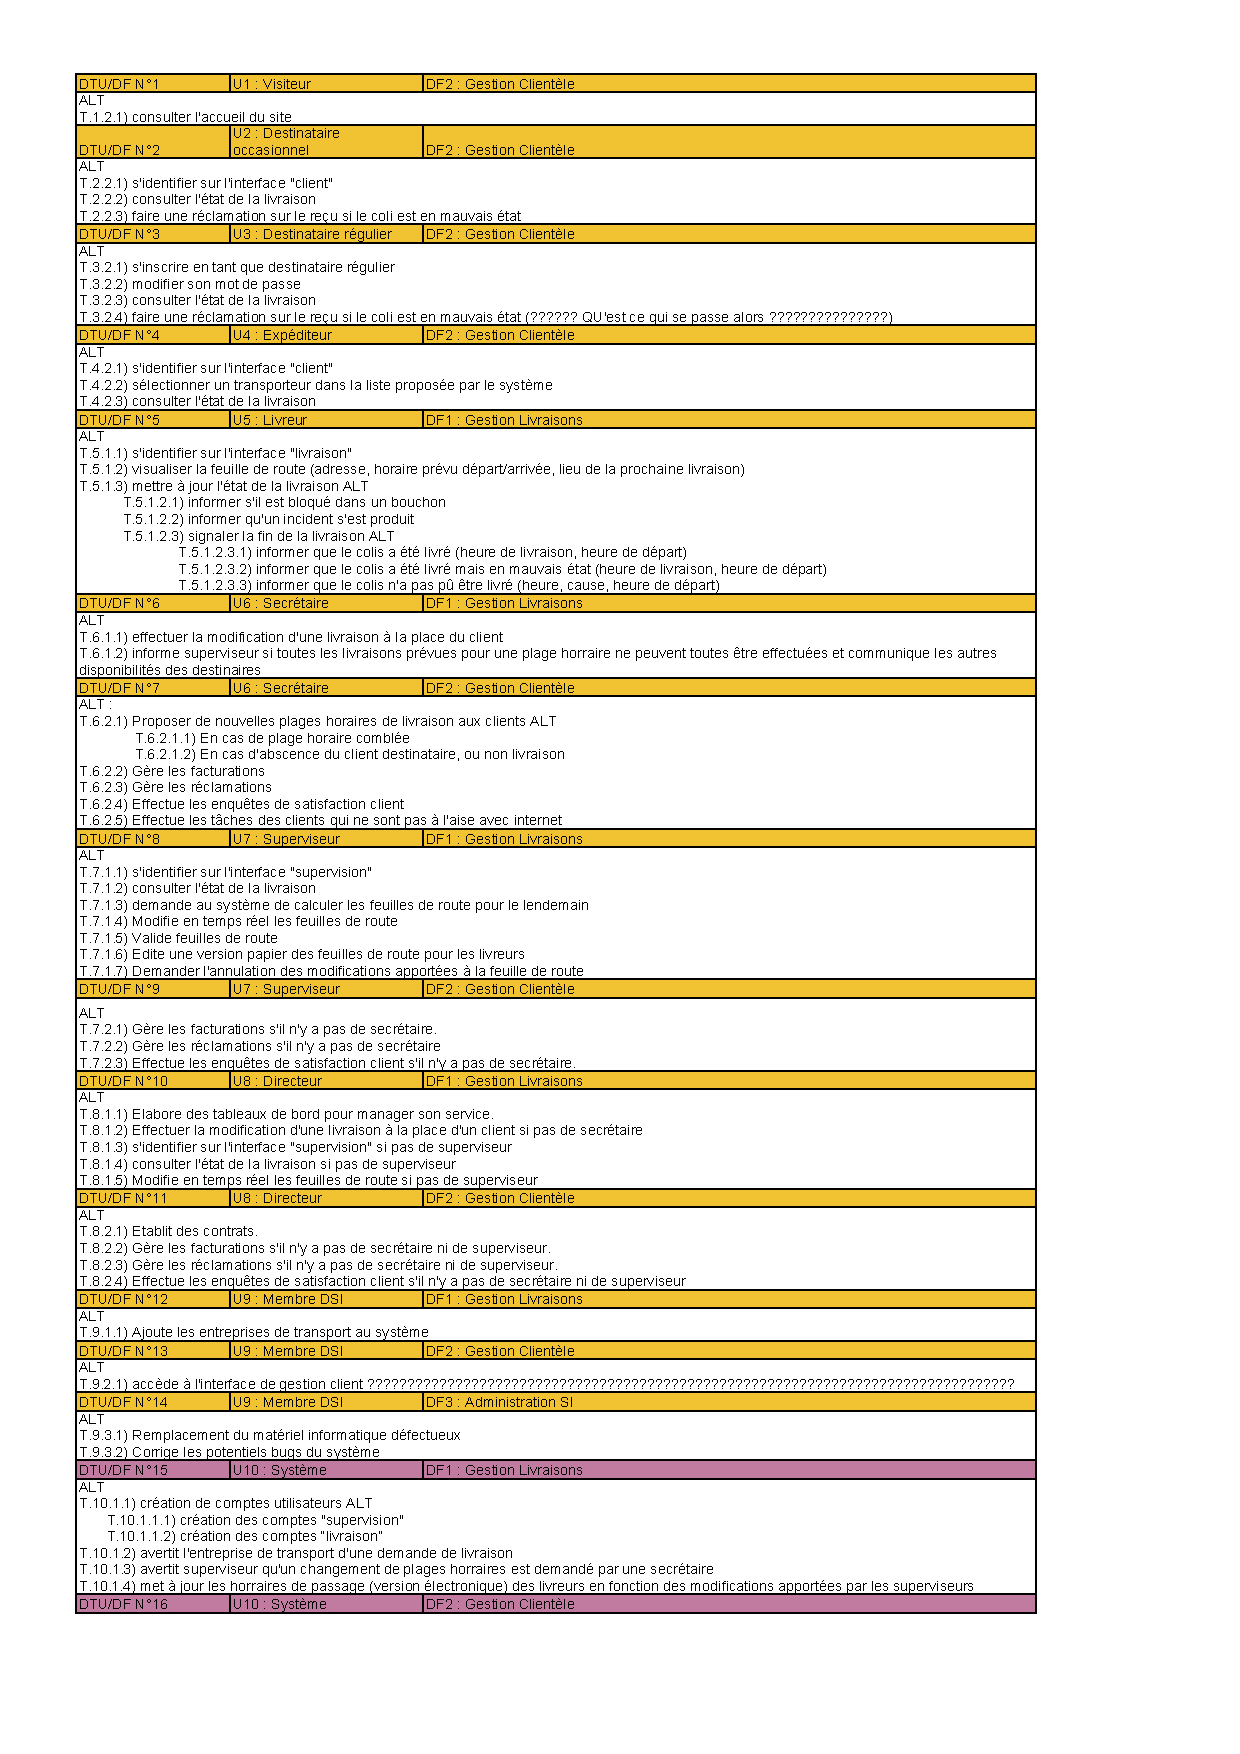
\includegraphics[scale = 0.7]{images/DTUDF.pdf}



%------------------DC-IHM------------------------%

\chapter{Description Conceptuelle de l'IHM}

\paragraph{}
Au cours de cette seconde partie de la conception d'OptiFret, nous avons une nouvelle fois séparé l'équipe en deux groupes de travail :\\
Equipe A : JM Comets, P Turpin, J Rollet\\
Equipe B : Q Coursodon, P Peller, M Paul\\


L'Equipe A a travaillé sur : DPOU, MSIHM\\

L'Equipe B s'est concentrée sur la partie suivante (Description Sémantique-IHM).\\

L’ensemble de l’équipe a travaillé sur : DICIHM\\

Cette seconde partie nous donne l'occasion d'extraire le travail effectué précédemment pour commencer à structurer notre future IHM autour de concepts donnés et précis. 

\section{Dossier d'Initialisation de la Conception de l'IHM}

\subsection{Charte graphique et Guide de style utilisé : }

Nous allons utiliser les deux documents qui nous ont été fournis par la COURLY, et qui sont “charte$\_$graphique$\_$COURLY” pour la charte graphique, et “guide$\_$style$\_$COURLY” pour le guide de style. Ainsi, nous respecterons l’aspect générale de l’application ayant été définie par le client.

\subsection{Ensemble des métaphores : }

\paragraph{Superviseur :}
~~\\
Le superviseur demande au système de calculer les feuilles de routes pour les livraisons du lendemain.\\
Le superviseur modifie la feuille de route en cas de livraisons impossible.\\
Le superviseur peut modifier interactivement les feuilles de route.\\
Le superviseur peut demander une mise à jour des horaires de passage au système.\\
Le superviseur voit les livraisons pour lesquelles la plage horaire ne respecte plus celle demandée par le client.\\
Le superviseur peut annuler les modifications apportées aux feuilles de route.\\
Le superviseur valide des feuilles de route.\\
Le superviseur édite une version papier.\\
Le superviseur observe l’état des livraisons en cours. \\
Le superviseur regarde en détail les informations concernant une livraison (effectuée ou non).\\
Le superviseur modifie la feuille de route d’un livreur (suppression d’une livraison, interversion de l’ordre de deux livraisons, ...).\\
Le superviseur demande au système de re-calculer les feuilles de routes pour les livraisons du lendemain.\\

\paragraph{Livreur :}
~~\\
Le livreur reçoit une version papier de sa feuille de route de la journée.\\
Le livreur visualise sa feuille de route pour la journée.\\
Le livreur visualise les informations détaillées d’une livraison à effectuer dans la journée (l’adresse de livraison, l’heure prévue d’arrivée à cette adresse, l’heure prévue de départ de cette adresse pour le prochain lieu de livraison, les coordonnées d’une personne à contacter en cas de problème).\\
Le livreur peut signaler s’il est bloqué dans un embouteillage.\\
Le livreur peut indiquer qu’il a effectué la livraison et remplir les informations concernant celle-ci (heure de livraison, heure de départ, livraison effectuée ou non - et dans ce dernier cas la cause).\\

\paragraph{Secrétaire :}
~~\\
La secrétaire contact les clients qui possèdent une livraison impossible pour leur proposer une nouvelle plage horaire.\\
La secrétaire informe le superviseur quand il y a des livraisons impossibles.\\

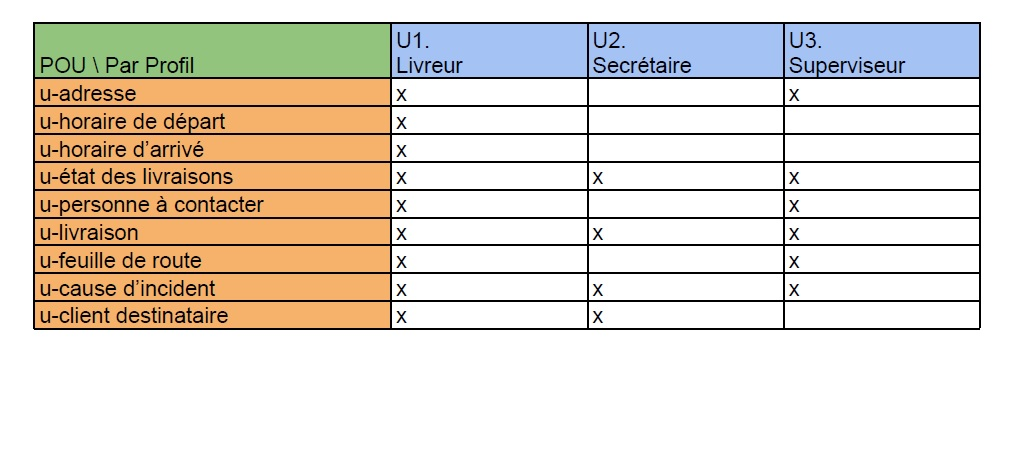
\includegraphics[scale = 0.5]{images/DICIHM.jpg}

\section{Modèle Structurel de l'IHM}

\subsection{Livreur : }
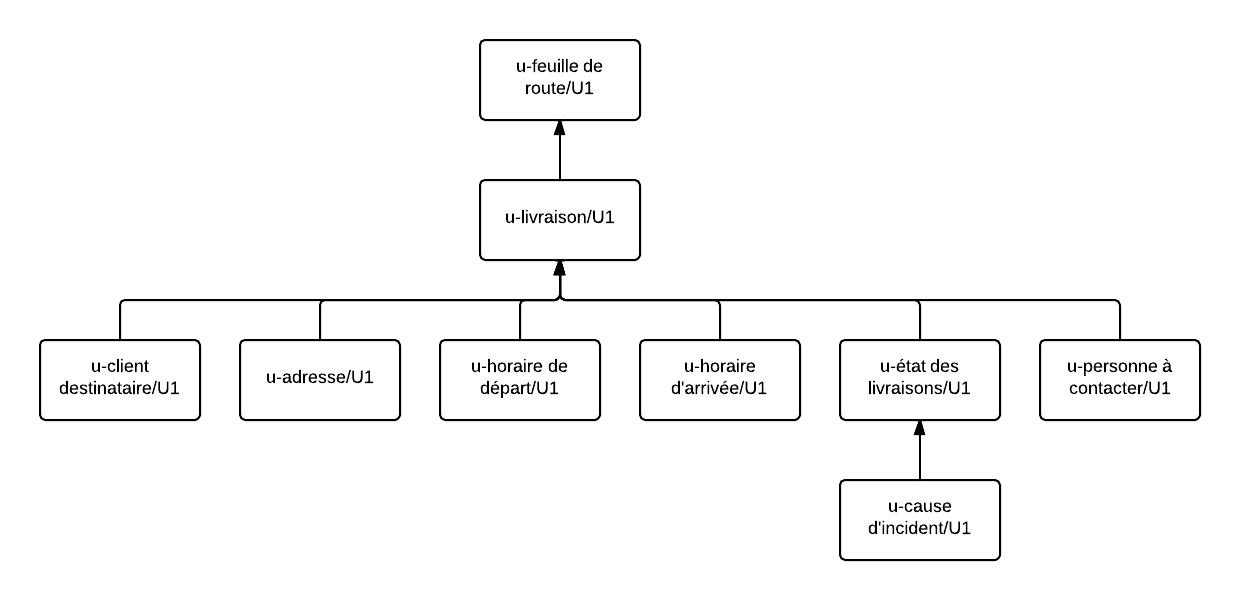
\includegraphics[scale = 0.33]{images/MSIHM-U1.jpeg}

\subsection{Secrétaire : }
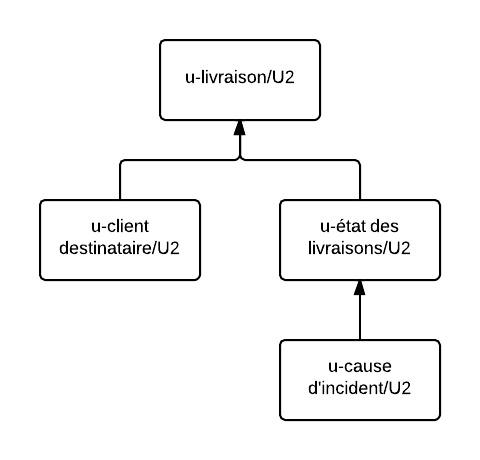
\includegraphics[scale = 0.4]{images/MSIHM-U2.jpeg}

\subsection{Superviseur  : }
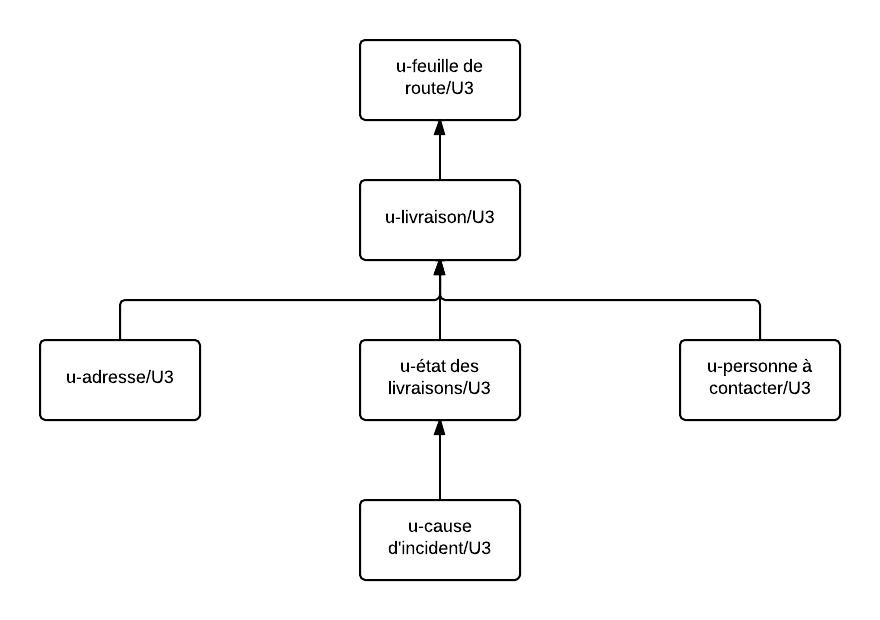
\includegraphics[scale = 0.4]{images/MSIHM-U3.jpeg}

\section{Description détaillée des Principaux Objets Utilisateurs}

\hypertarget{labDPOU}{}

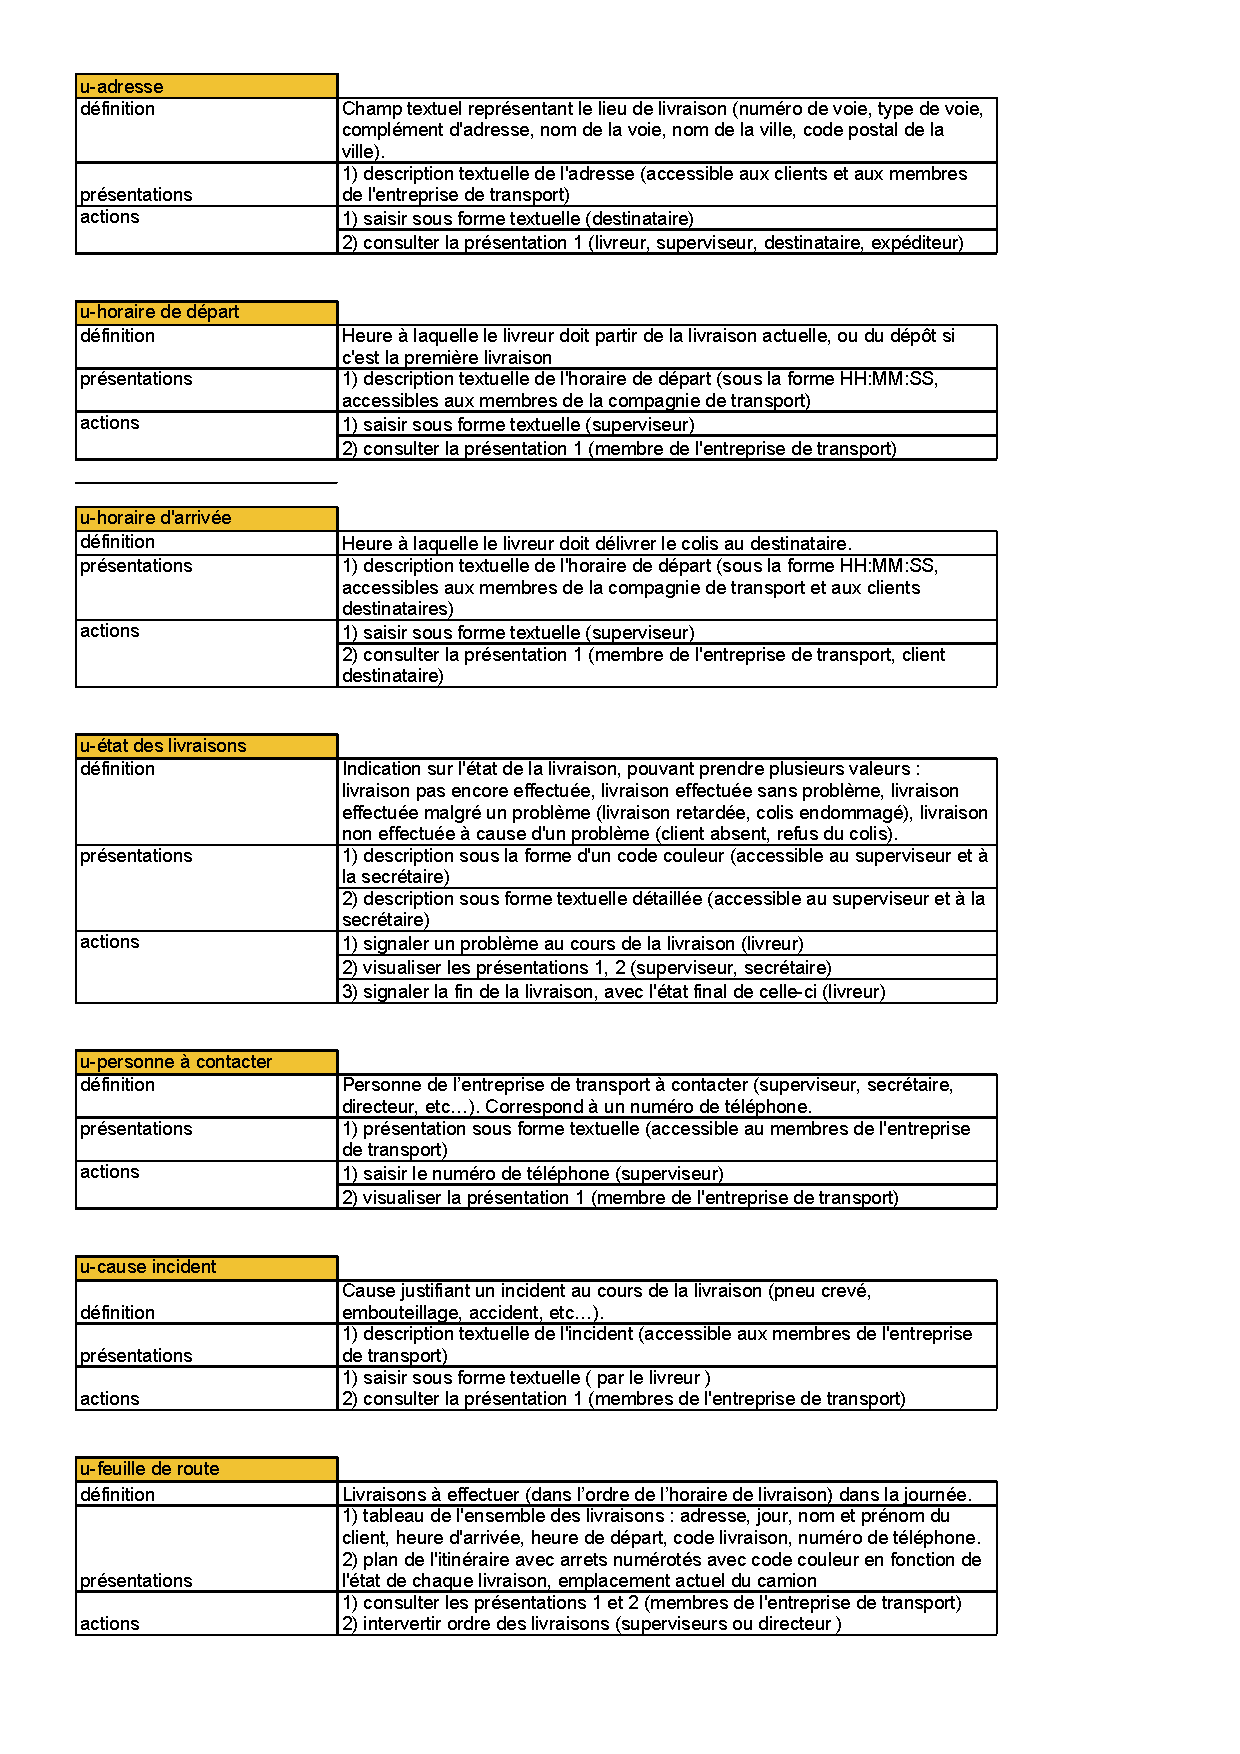
\includegraphics[scale = 0.65, page = 1]{images/DPOU.pdf} 

\includegraphics[scale = 0.7, page = 2]{images/DPOU.pdf}

%------------------DS-IHM------------------------%

\chapter{Description de la Sémantique de l'IHM}

\paragraph{}
Cette troisième partie a été effectuée au sein de la même séance que la partie précédente, donc les équipes de travail n'ont pas été modifiées.\\

L'Equipe B a travaillé sur : DAU, PHTU-A\\

L'ensemble de l'équipe a travaillé sur : TC / U, TU / C et D-COM\\

Cet ensemble de descriptions permet la concrétisation précise des commandes à implémenter, données pour un ou plusieurs utilisateurs.

\newpage

\section{Planification Hiérarchique de la Tâche Utilisateur Approfondie}

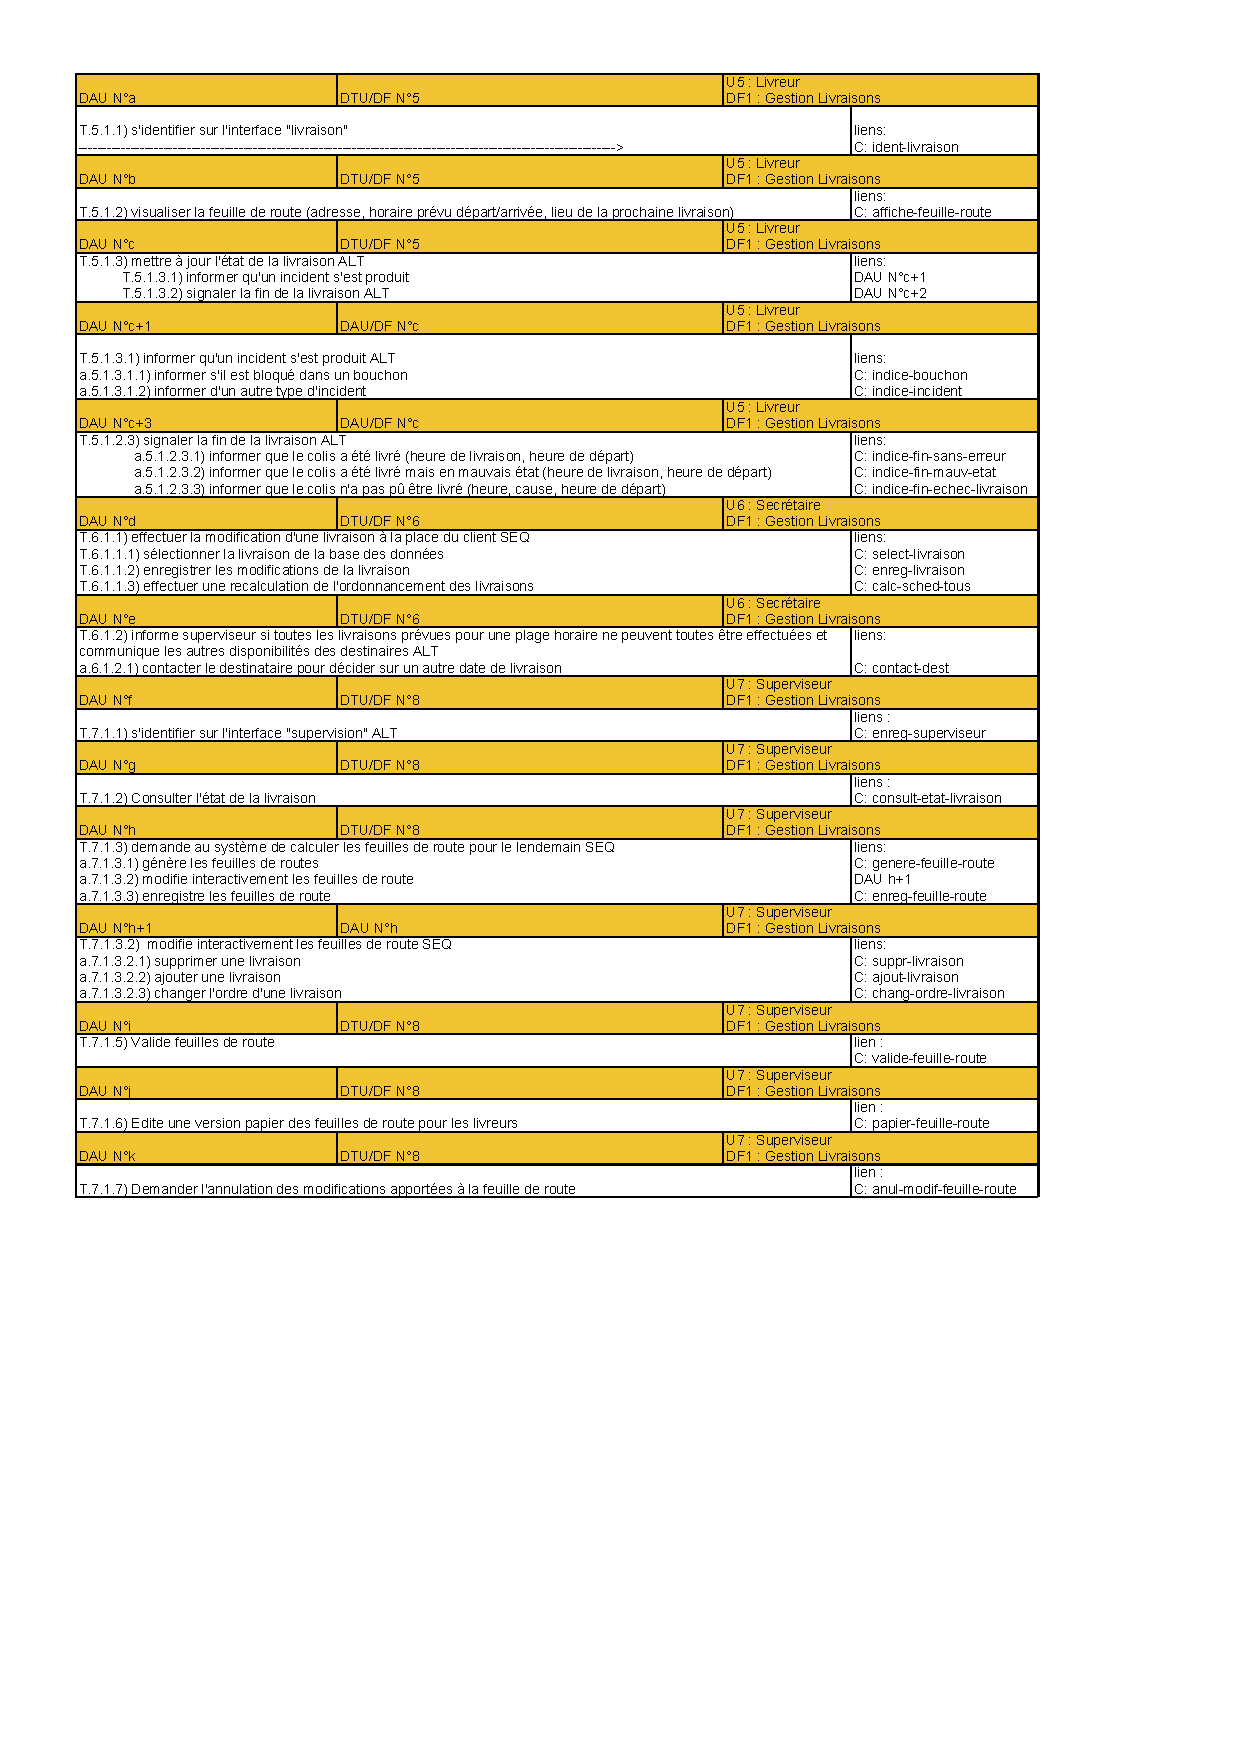
\includegraphics[scale = 0.85]{images/DAU.pdf}

\section{Table des Commandes par Utilisateurs}

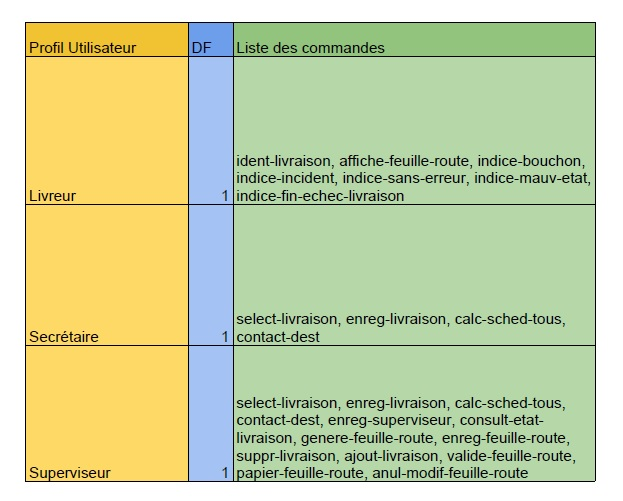
\includegraphics[scale = 0.6]{images/TCU.jpg}

\section{Table des Utilisateurs par Commande}

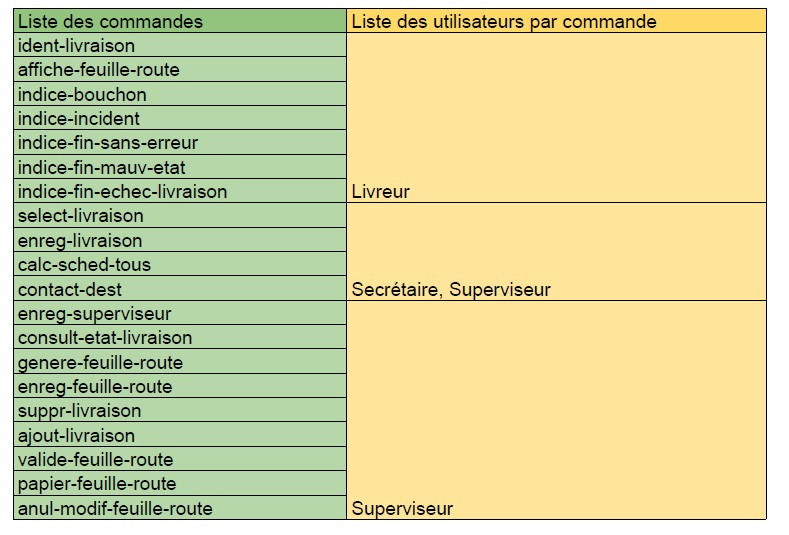
\includegraphics[scale = 0.6]{images/TUC.jpg}

\section{Description des COMmandes}

\hypertarget{labDCOM}{}

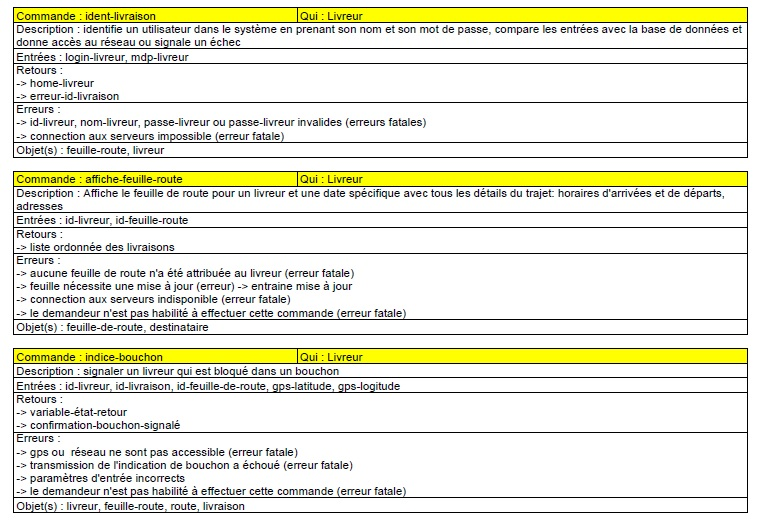
\includegraphics[scale = 0.7]{images/DCOM0.jpg}\\
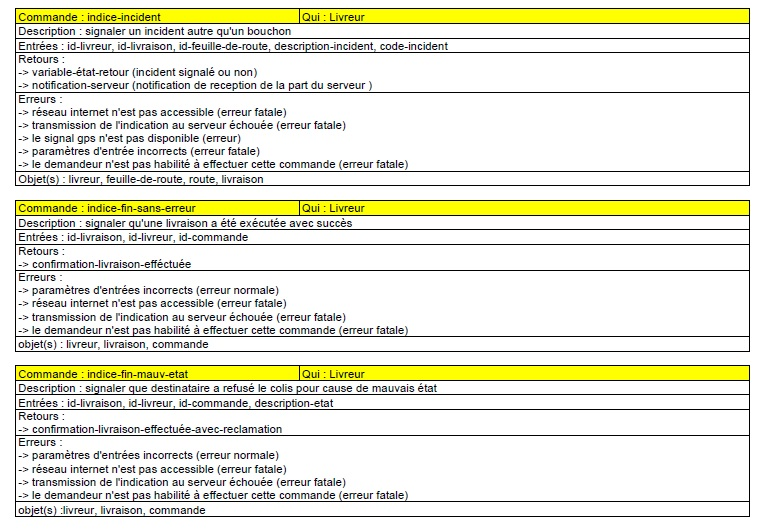
\includegraphics[scale = 0.7]{images/DCOM1.jpg}\\
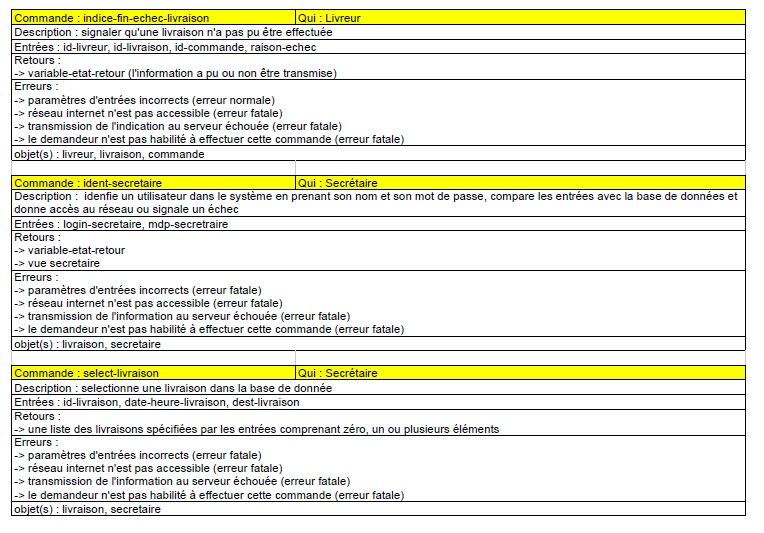
\includegraphics[scale = 0.7]{images/DCOM2.jpg}\\
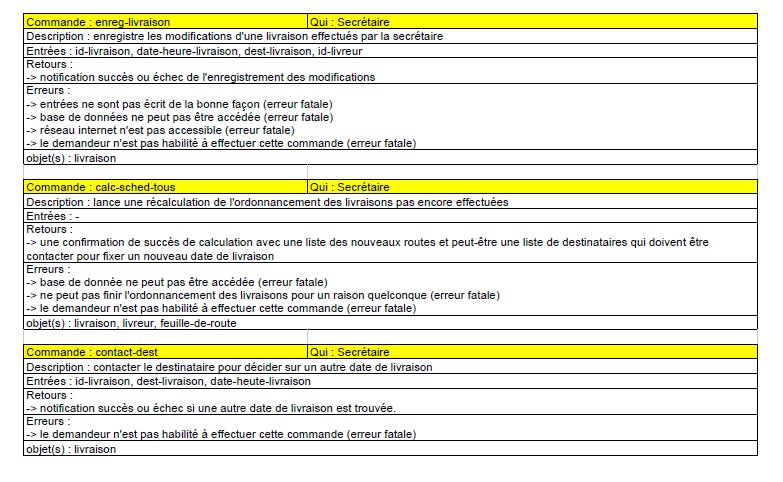
\includegraphics[scale = 0.7]{images/DCOM3.jpg}\\
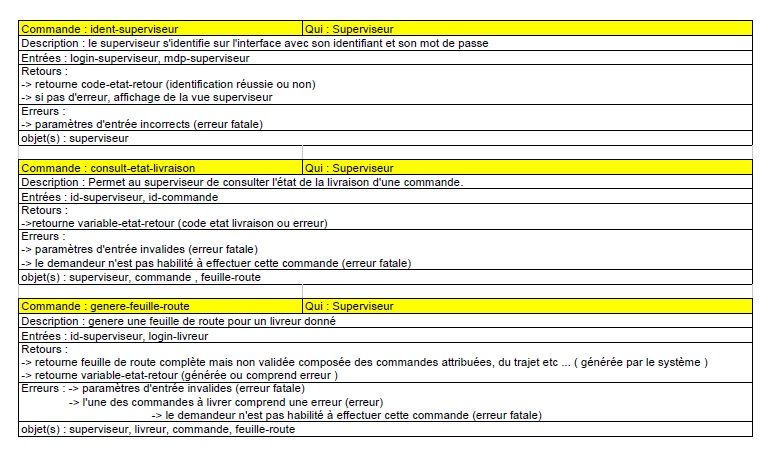
\includegraphics[scale = 0.7]{images/DCOM4.jpg}\\
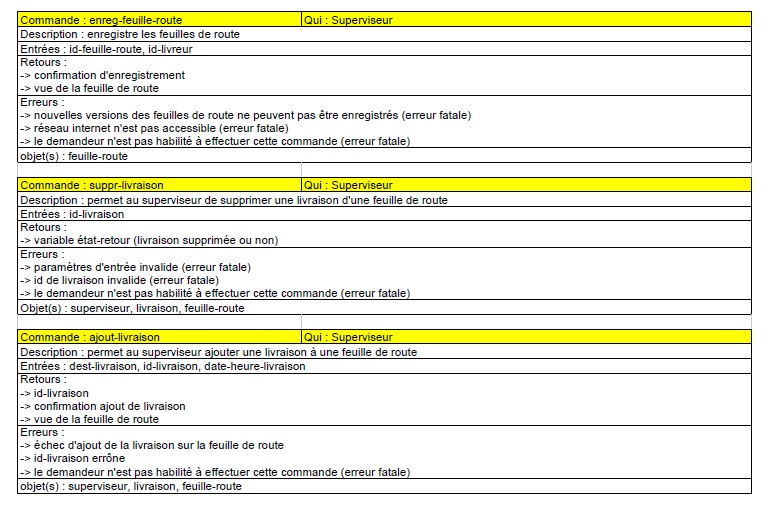
\includegraphics[scale = 0.7]{images/DCOM5.jpg}\\
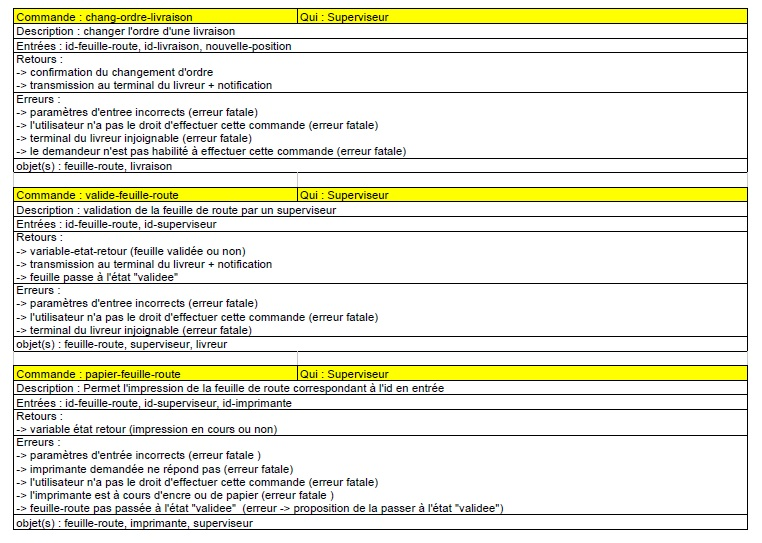
\includegraphics[scale = 0.7]{images/DCOM6.jpg}\\
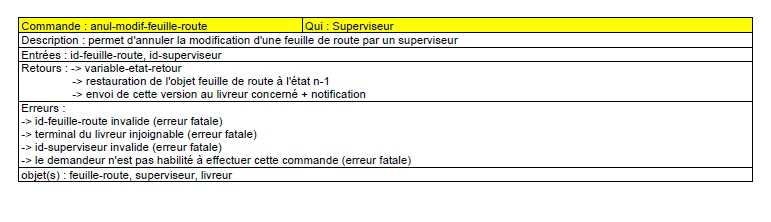
\includegraphics[scale = 0.7]{images/DCOM7.jpg}\\


%-----------------DSy-IHM------------------------%

\chapter{Description Syntaxique de l'IHM}


\section{Spécification Syntaxique du Langage d'Entrée / de Sortie}

\paragraph{Entrées :}
~~\\
e-ident-livraison :: edb-il, identifiant-livreur, efn-il\\
identifiant-livreur :: id-livreur, mdp-livreur\\
~~\\
e-indice-bouchon :: edb-ib, info-indice, gps-position, efn-ib\\
e-indice-incident :: edb-ii, info-indice, code-incident, description-incident, efn-ii\\
info-indice :: id-livreur, id-livraison, id-feuille-route\\
gps-position :: gps-latitude, gps-position\\
~~\\
e-indice-fin :: edb-if, e-livraison, id-commande, etat-fin | “OK”, description-etat-fin?, efn-if\\
~~\\
e-select-livraison :: edb-sl, livraison, efn-sl\\
e-enreg-livraison :: edb-el, livraison, id-livreur, efn-el\\
e-contact-dest :: edb-cd, livraison, efn-db\\
livraison :: id-livraison, dest-livraison, date-heure-livraison\\
~~\\
e-calc-sched-tous :: edb-cst, efn-cst\\
~~\\
e-enreg-superviseur :: edb-es, identifiant-superviseur, edb-es\\
identifiant-superviseur :: nom-superviseur, mdp-superviseur\\
~~\\
e-consult-etat-livraison :: edb-cel, id-superviseur, id-commande, efn-cel\\
e-genere-feuille-route :: edb-gfr, id-superviseur, login-livreur, efn-gfr\\
e-enreg-feuille-route :: edb-efr, id-feuille-route, id-livreur, efn-efr\\
~~\\
e-ajout-livraison :: edb-al, livraison, efn-al\\
e-suppr-livraison :: edb-fl, id-livraison, efn-sl\\
~~\\
e-chang-ordre-livraison :: edb-col, id-feuille-route, id-livraison, nouvelle-position, efn-col\\
e-valide-feuille-route :: edb-vfr, id-feuille-route, id-superviseur, efn-vfr\\
e-papier-feuille-route :: edb-pfr, id-feuille-route, id-superviseur, id-imprimante, efn-pfr\\
e-anul-modif-feuille-route :: edb-amfr, id-feuille-route, id-superviseur, efn-amfr\\

\paragraph{Sorties :}
~~\\
r-erreur-ident-livraison :: rdb-eil, r-action-confi-erreur | r-action-abort, rfb\\
home-livreur :: \\
r-affiche-feuille-route :: livraison*\\

La DTD tirée de ce ... est présente en Annexe \ref{labDTD}.

\section{Diagramme d'Enchaînement des Fenêtres}

\paragraph{}
~~\\
\begin{center}
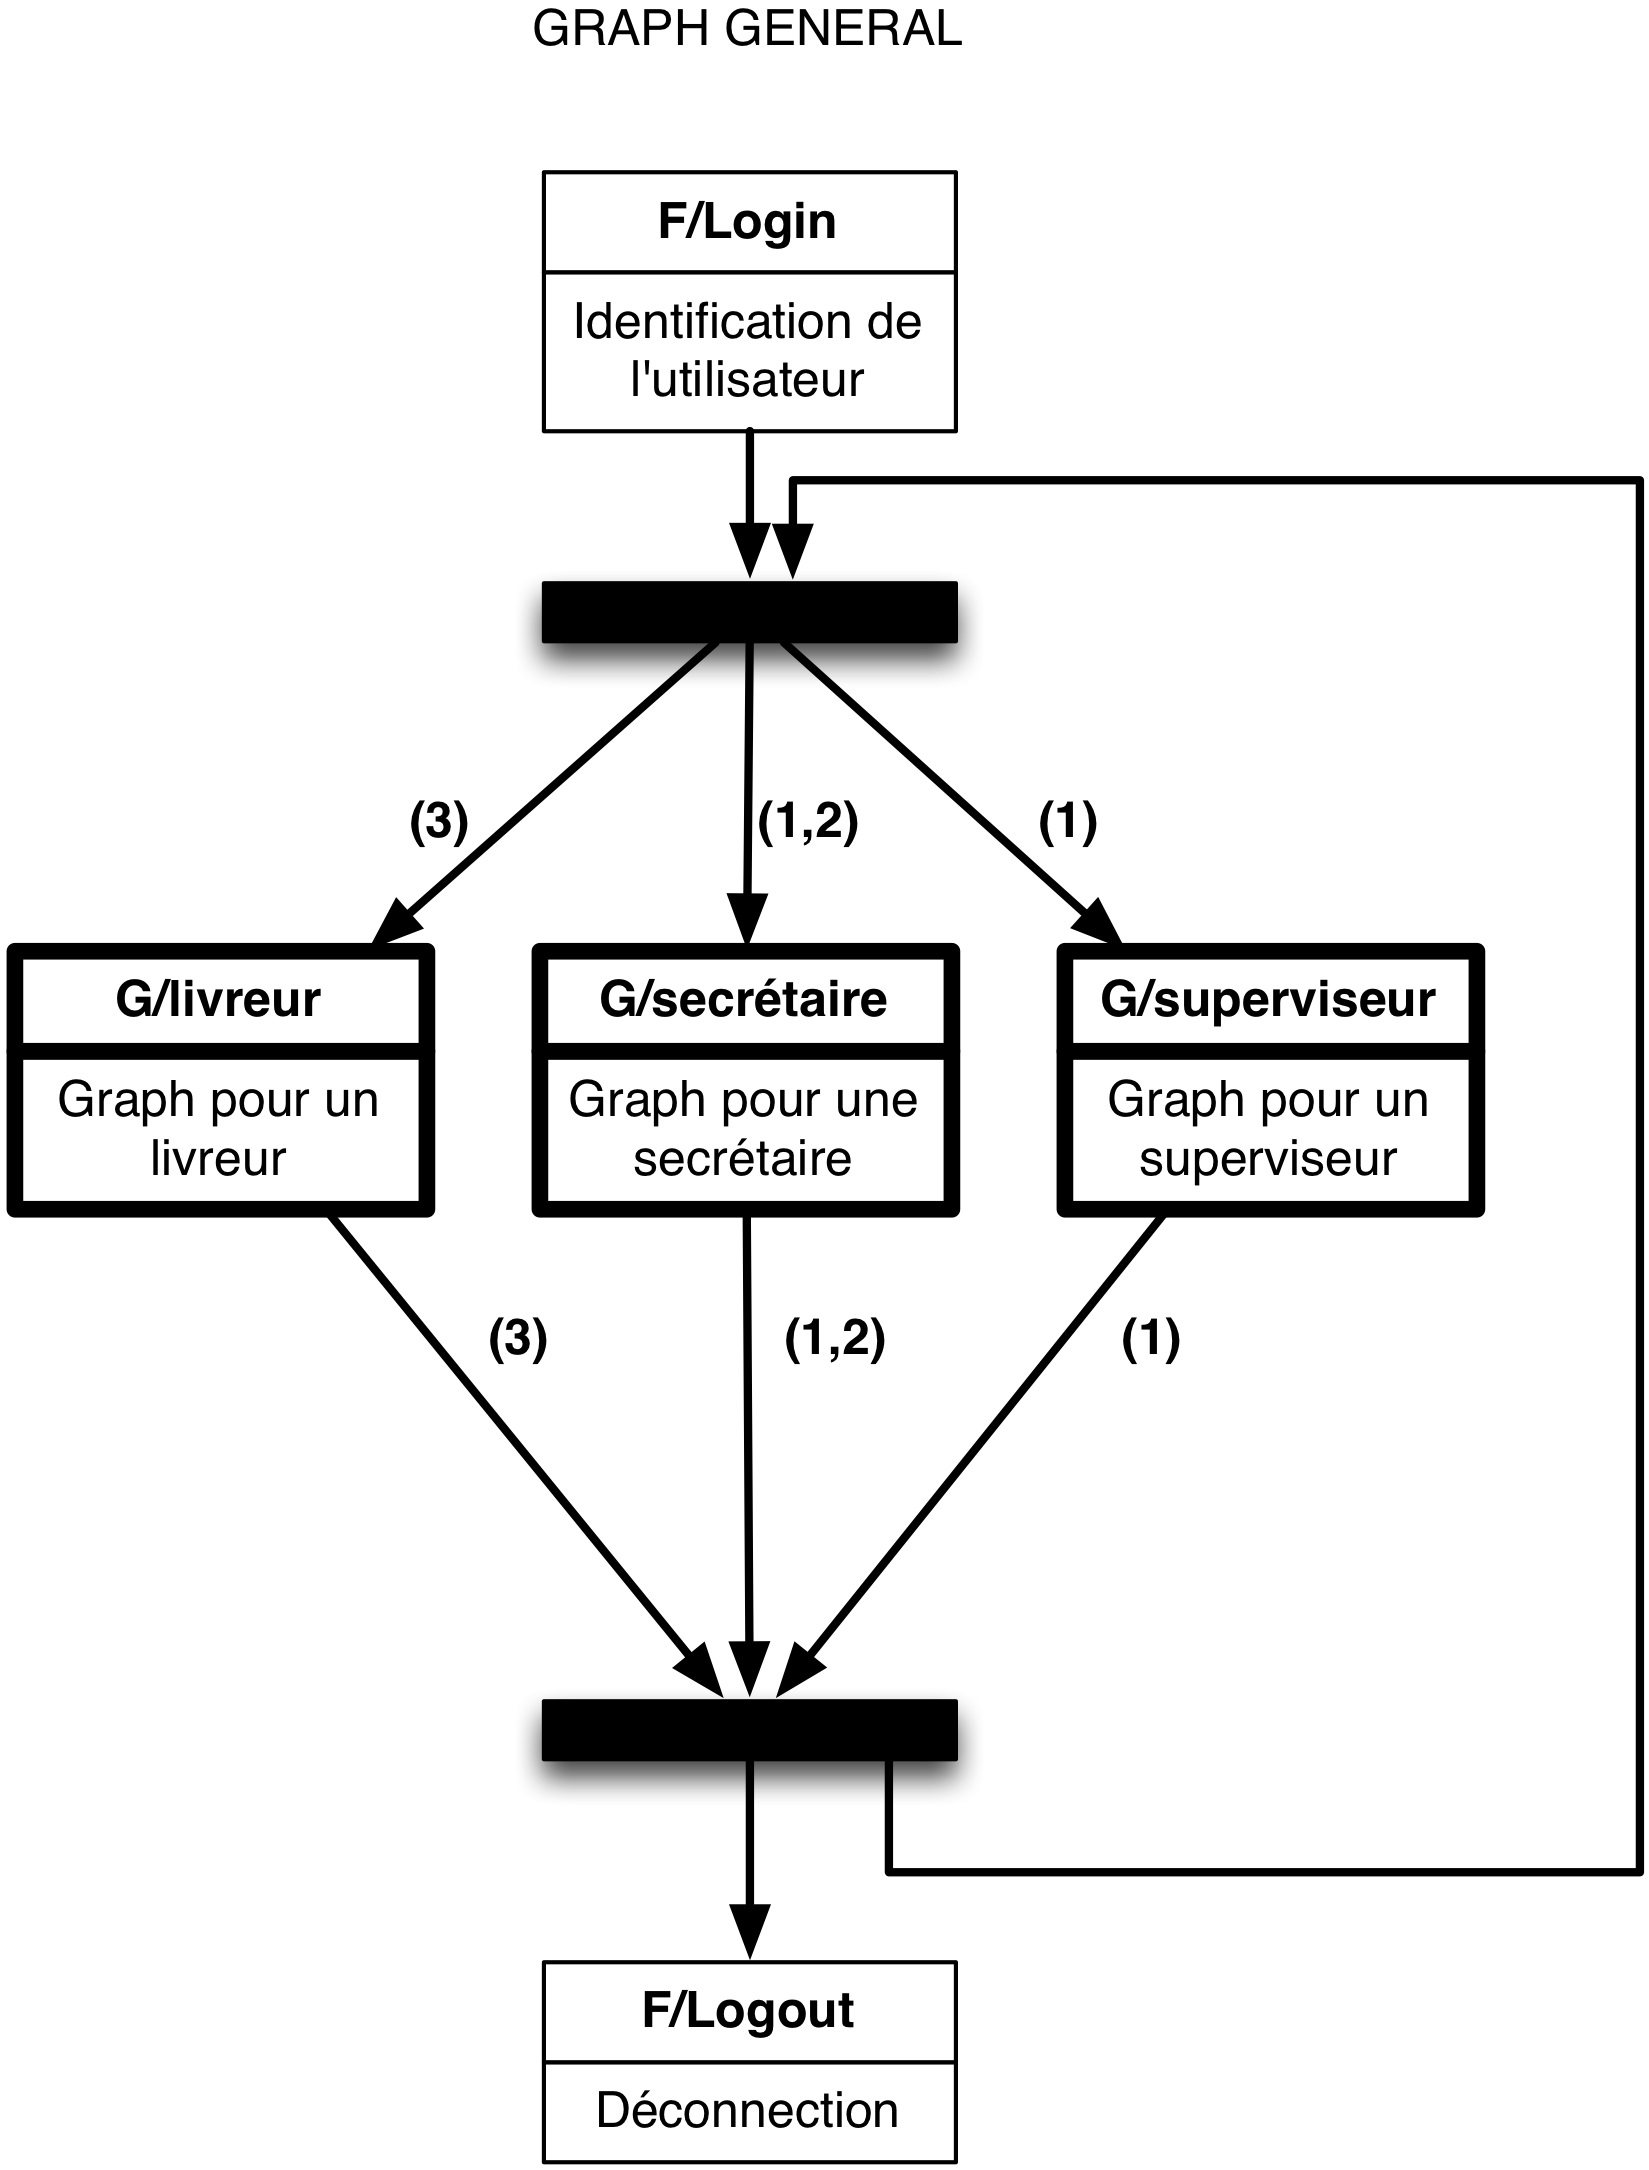
\includegraphics[scale = 0.18]{images/general.jpg}
\end{center}

\paragraph{}
~~\\
\begin{center}
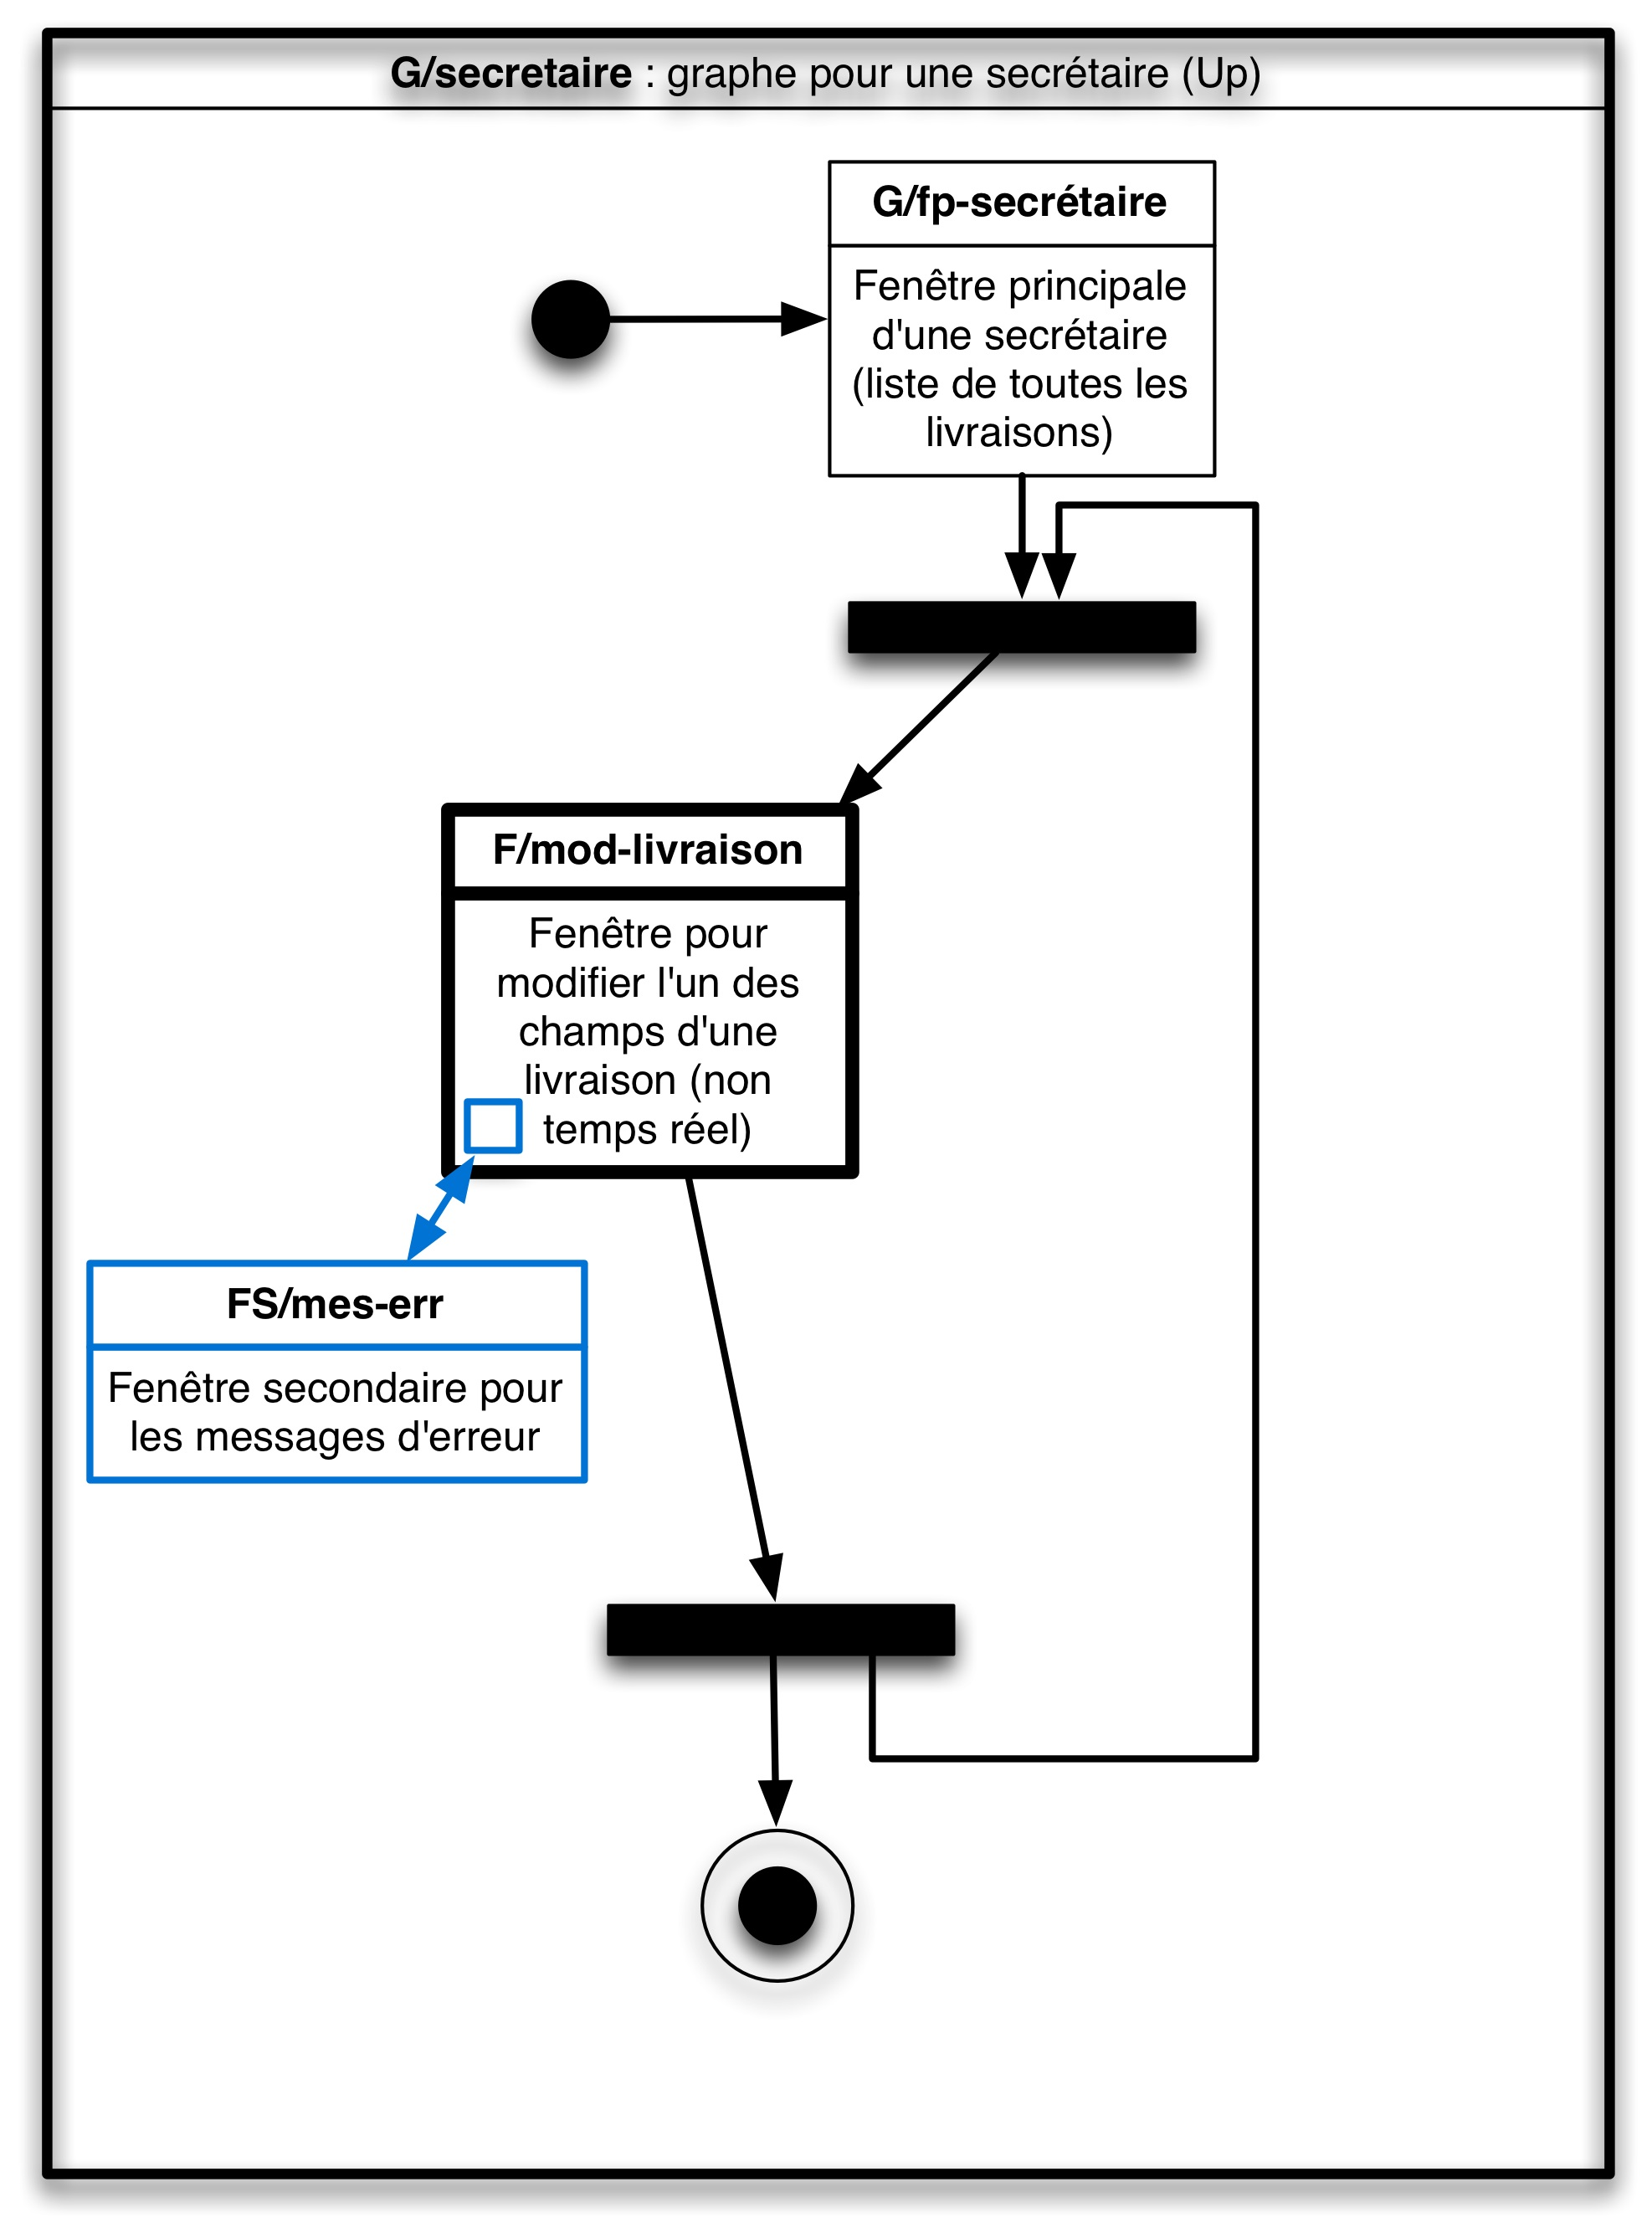
\includegraphics[scale = 0.25]{images/g-secretaire.jpg}
\end{center}

\paragraph{}
~~\\
\begin{center}
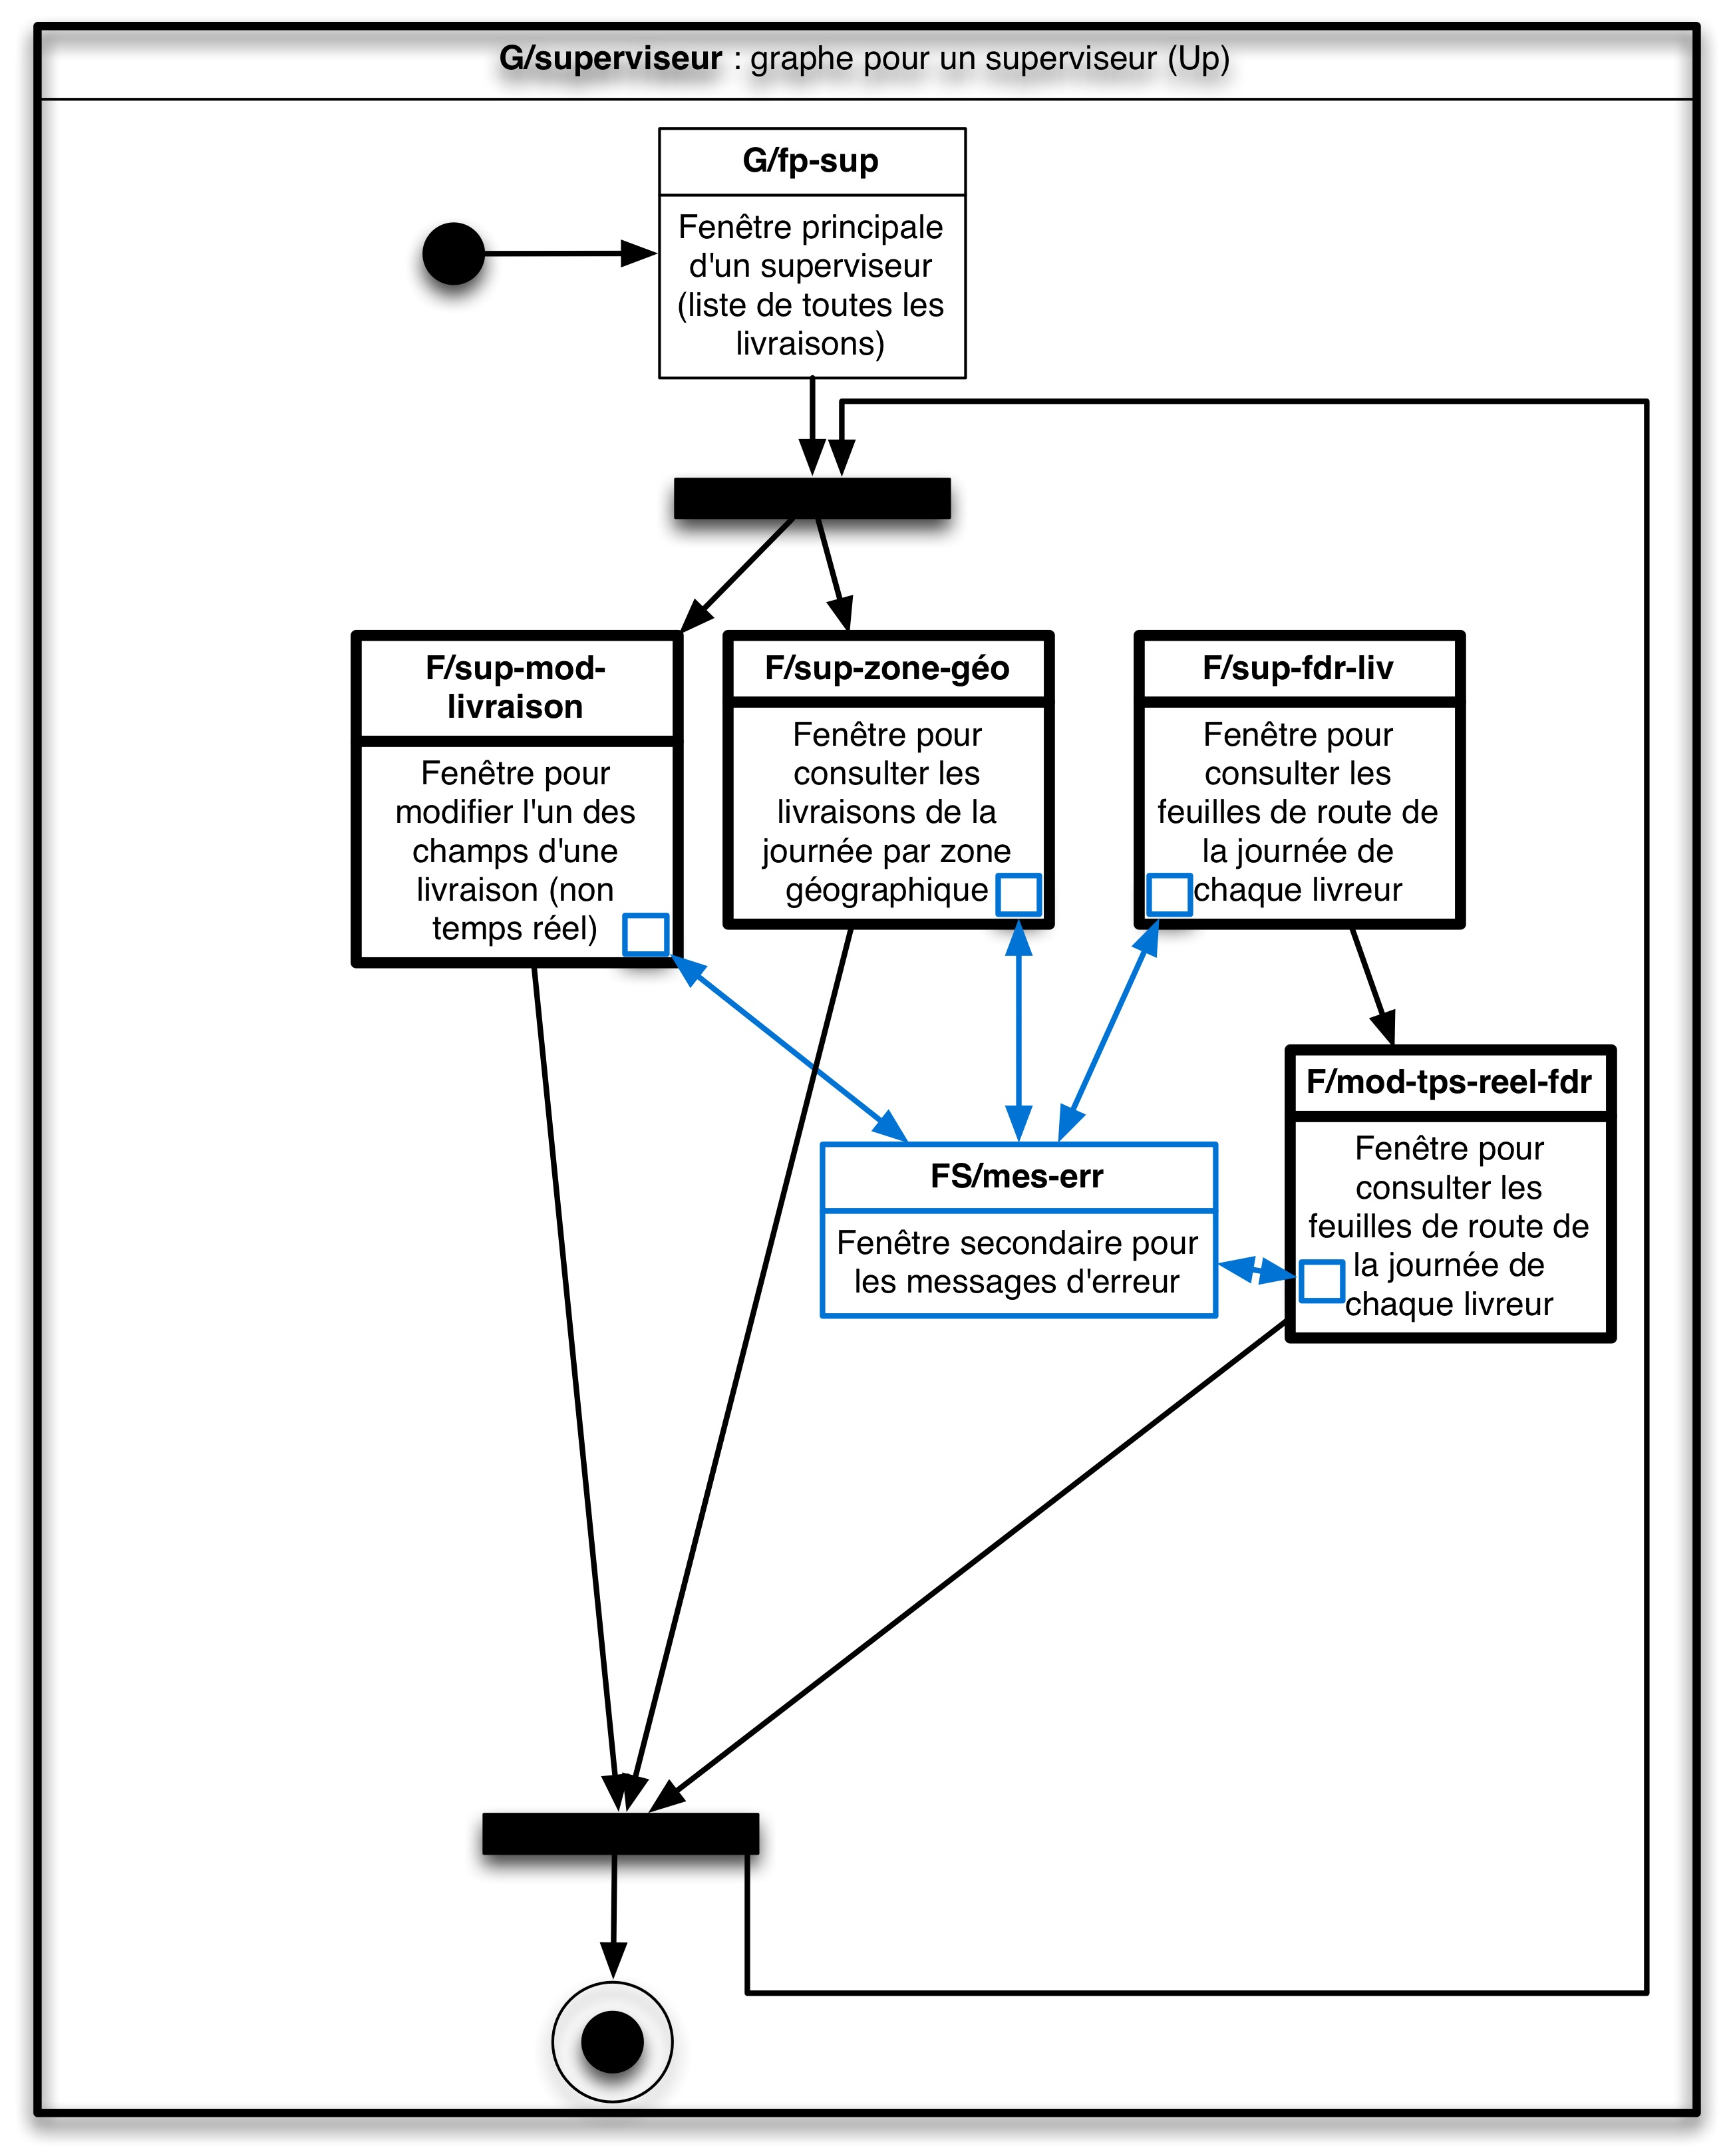
\includegraphics[scale = 0.2]{images/g-sup.jpg}
\end{center}

\paragraph{}
~~\\
\begin{center}
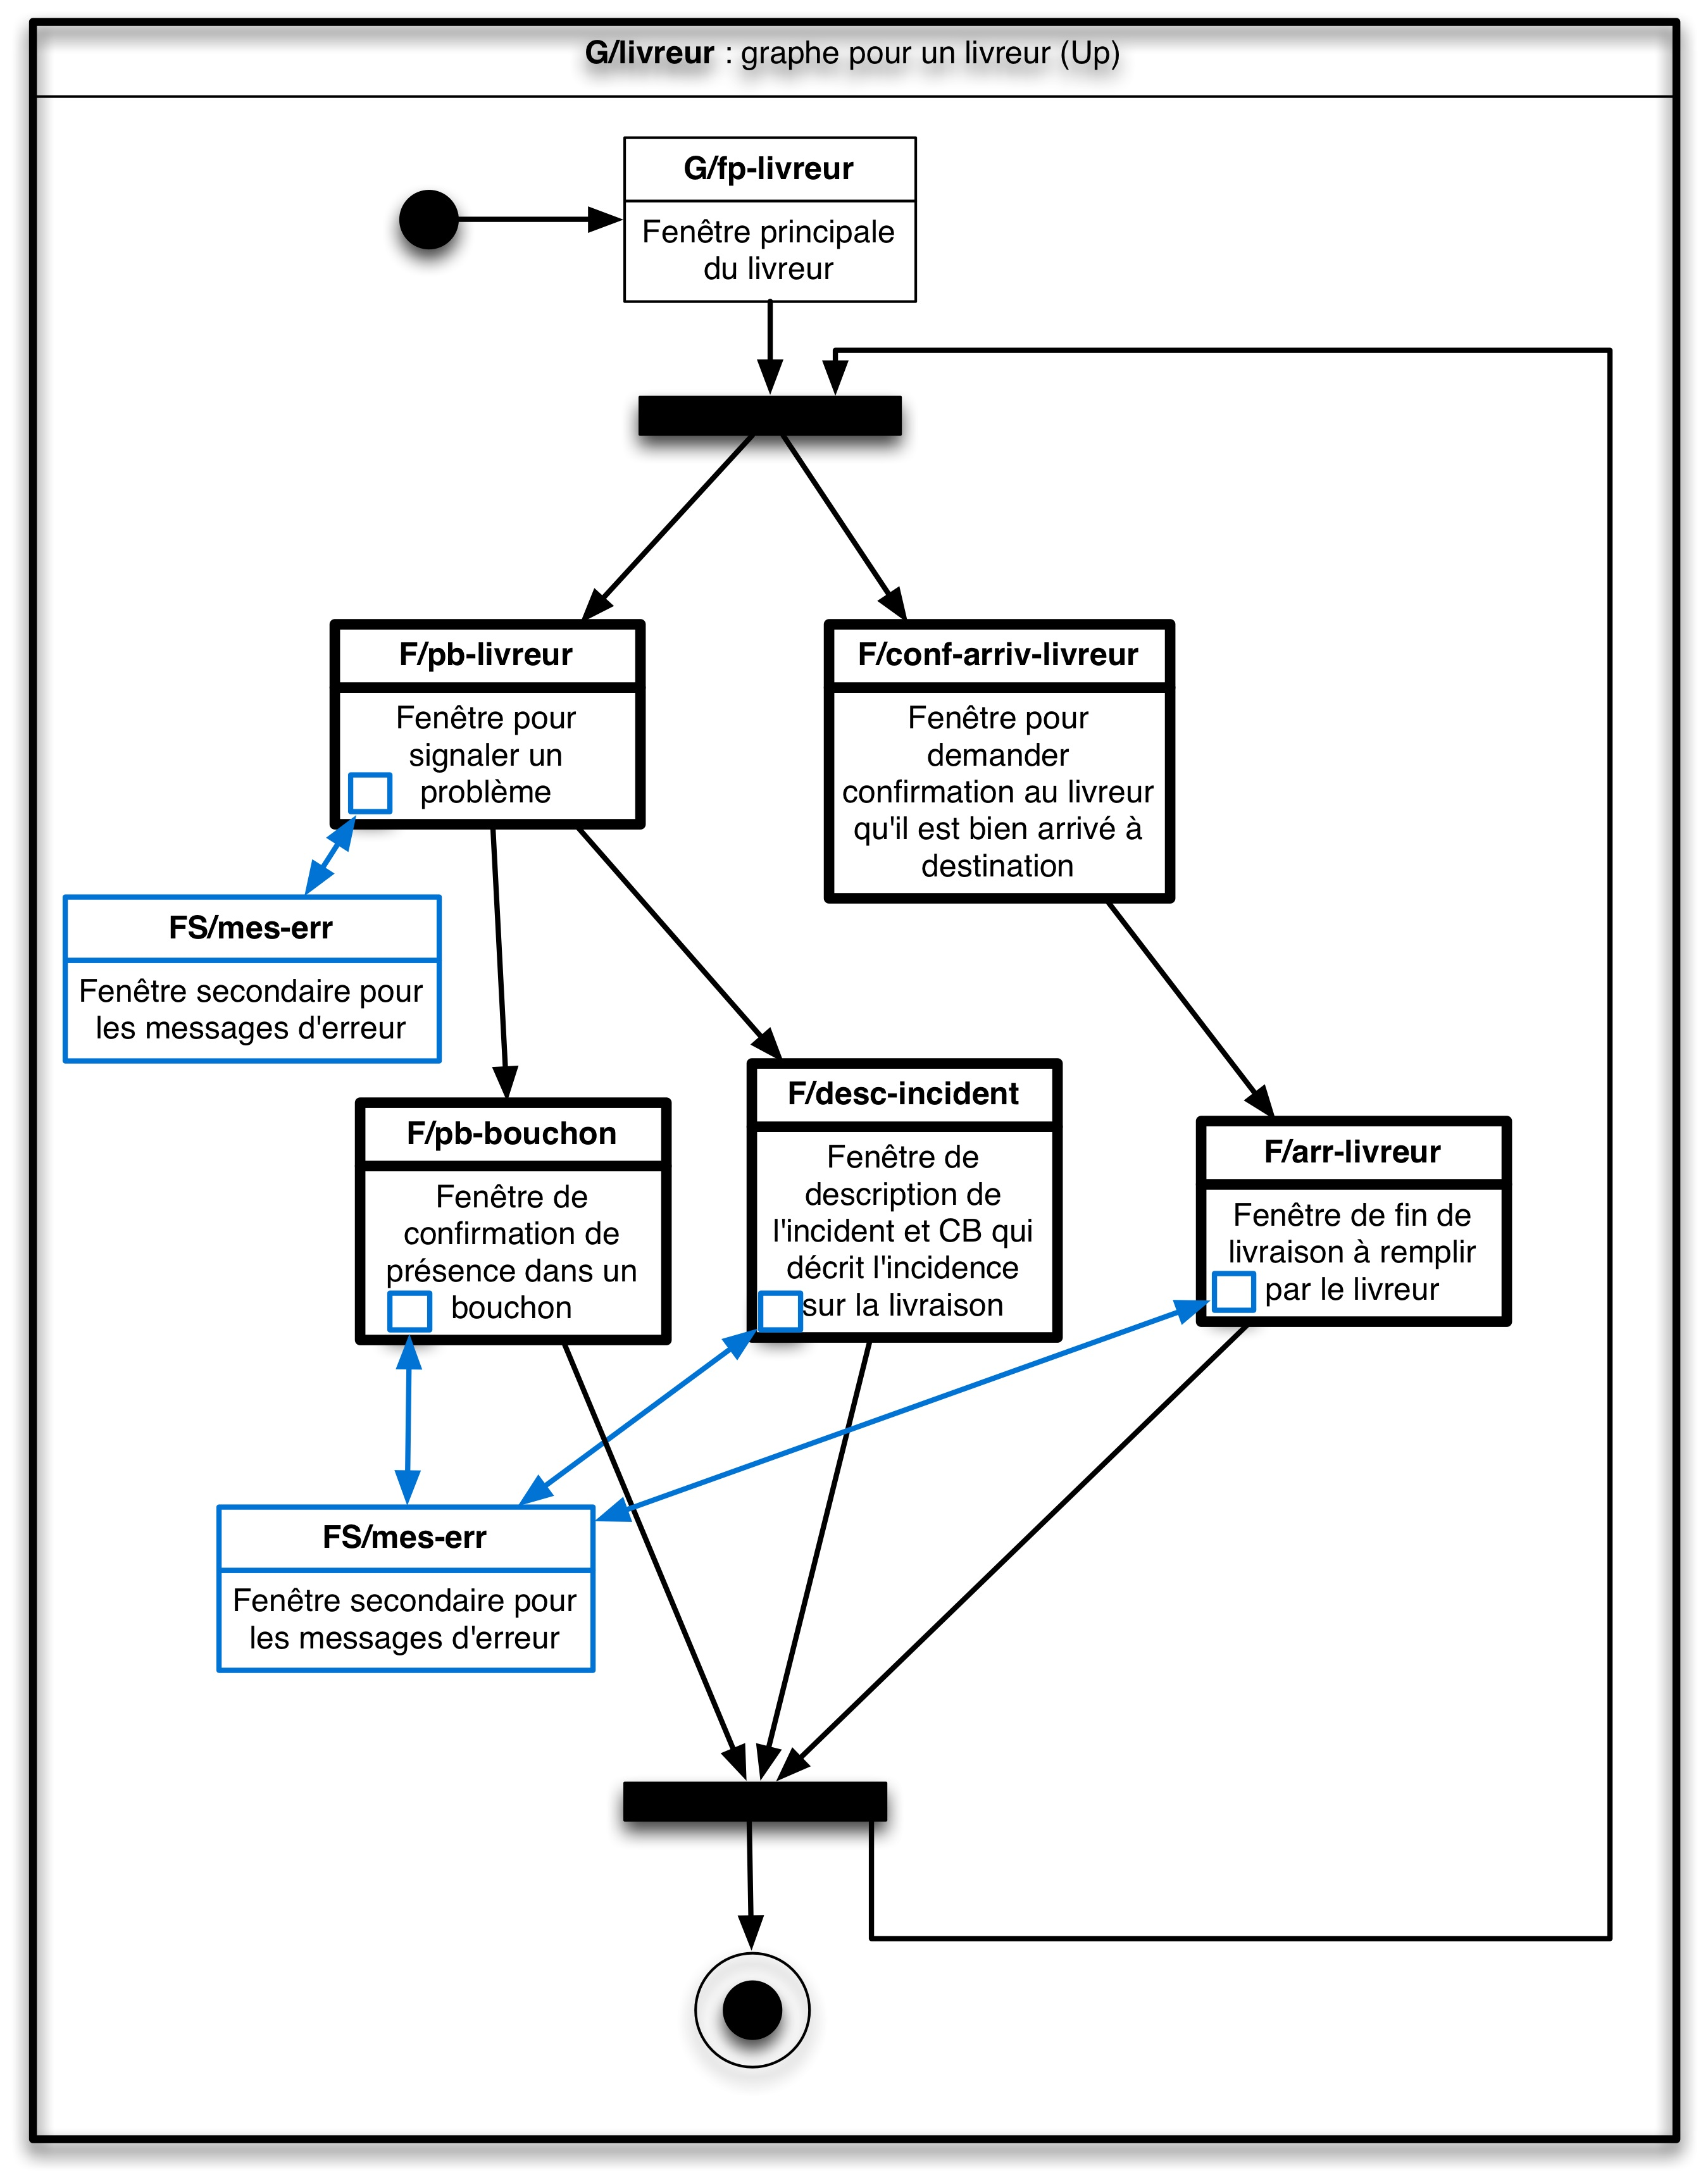
\includegraphics[scale = 0.2]{images/g-livreur.jpg}
\end{center}

\section{Diagramme d'Etats des Classes}





%------------------DL-IHM------------------------%

\chapter{Description Lexicale de l'IHM}


\section{Lexique des Objets Graphiques}

\begin{longtable}{|p{5cm}|p{5cm}|c|}
\hline
Identificateur&Description&Dessin\\\hline
secr-modif-select-livraison&Zone de saisie permettant le choix de la livraison à modifier&
\includegraphics{images/tools.png}\\\hline
secr-modif-zone-adresse&Zone de saisie de l'adresse de destination de la livraison&\\\hline
secr-modif-zone-urgence&Zone de saisie de la personne à contacter en cas d'urgence pendant la livraison&\\\hline
secr-modif-zone-date&Zone de saisie de la date de la livraison&\\\hline
secr-modif-zone-heure&Zone de saisie de l'heure de la livraison&\\\hline
secr-modif-btn-validation&Bouton de validation des modifications de la livraison&\\\hline
secr-modif-calendrier&Calendrier de choix d'une date aidant la saisie de la date de la livraison&\\\hline
sup-modif-select-feuille-route&Liste déroulante de choix de la feuille de route à visualiser/modifier&\\\hline
sup-modif-liste-livraison&Liste des livraisons ordonnées à faire pour la feuille de route choisie&\\\hline
sup-modif-livraison&Element coloré de la liste des livraisons&\\\hline
sup-modif-livraison-ico-suppr&Icône de suppression de la livraison&\\\hline
sup-modif-livraison-ico-deroul&Icône de déroulement des informations détaillées sur la livraison&\\\hline
sup-modif-livraison-ico-enroul&Icône d'enroulement des informations détaillées sur la livraison&\\\hline
sup-modif-livraison-txt-adresse&Etiquette indiquant l'adresse de livraison&\\\hline
sup-modif-livraison-txt-heure-arrive&Etiquette indiquant l'heure d'arrivé de la livraison&\\\hline
sup-modif-livraison-txt-heure-depart&Etiquette indiquant l'heure de départ de la livraison&\\\hline
sup-modif-livraison-txt-itineraire&Etiquette indiquant l'itinéraire à suivre pour livrer le colis&\\\hline
sup-modif-livraison-txt-urgence&Etiquette indiquant la personne à contacter en cas d'urgence&\\\hline
sup-modif-map-vue&Vue aérienne de la carte de navigation.&\\\hline
sup-modif-map-ico-dest&Icône représentant un destinataire sur la carte de navigation.&\\\hline
sup-modif-map-ico-livreur&Icône représentant le livreur sur la carte de navigation&\\\hline
sup-modif-map-ico-depot&Icône représentant le dépôt sur la carte de navigation&\\\hline
livreur-heure-courante&"Affichage de l'heure courante, changeant en temps réel."&\\\hline
livreur-heure-arrivée&Affichage de l'heure d'arrivée prévue.&\\\hline
livreur-ico-probleme&"Icône représentant un incident, servant à accéder au dialogue "urgence"&\\\hline
livreur-adresse&Affichage de l'adresse du destinataire.&\\\hline
livreur-map-vue&Vue aérienne de la carte de navigation.&\\\hline
livreur-map-ico-dest&Icône représentant un destinataire sur la carte de navigation.&\\\hline
livreur-map-ico-livreur&Icône représentant le livreur sur la carte de navigation.&\\\hline
livreur-dial-urgence-numéro&"Affichage du numéro à appeler en cas d'urgence sur le dialogue "urgence"&\\\hline
livreur-dial-urgence-btn-incident&"Bouton servant au signalement d'un incident à partir du dialogue ""urgence"&\\\hline
livreur-dial-urgence-btn-bouchon&"Bouton servant au signalement d'un bouchon à partir du dialogue ""urgence"&\\\hline
livreur-dial-urgence-btn-fermer&"Bouton servant à fermer le dialogue ""urgence"&\\\hline
livreur-dial-bouchon&Dialogue permettant de confirmer si on est effectivement dans un bouchon.&\\\hline
livreur-btn-arrivé&Bouton servant à indiquer l'arrivée à la destination.&\\\hline
livreur-dial-incident-description&Zone de saisie décrivant l'incident rencontré.&\\\hline
livreur-dial-incident-état&Zone de sélection multiple permettant de sélectionner l'état après l'incident.&\\\hline
livreur-dial-incident-signaler&Groupe de boutons permettant de confirmer le signalement d'un incident.&\\\hline
livreur-dial-arrivé&Dialogue permettant de confirmer si on est effectivement arrivé.&\\\hline
livreur-radio-client-présent&Zone de sélection multiple permettant l'indiquer si le client était présent pour la livraison.&\\\hline
livreur-radio-livraison-effectuée&Zone de sélection multiple permettant l'indiquer si la livraison a été effectuée. Cet élément peut être désactivé et est grisé dans ce cas.&\\\hline
livreur-heure-livraison&Zone de saisie de l'heure de livraison, remplie par défaut avec l'heure à laquelle l'arrivée a été signalée.&\\\hline
livreur-txt-cause&Zone de saisie de la cause d'incident empêchant la livraison. Cet élément peut être désactivé et est grisé dans ce cas.&\\\hline
livreur-heure-départ&Affichage de l'heure de départ prévue pour la prochaine livraison. Cet affichage est coloré en rouge si l'heure est passée, en vert dans le cas contraire.&\\\hline
livreur-btn-départ&Bouton servant à signaler le départ d'un lieu de livraison, enclanchant la navigation pour la livraison suivante.&\\\hline
livreur-dial-départ&Dialogue servant à confirmer la saise d'informations sur la livraison actuelle pour lancer la navigation pour la livraison suivante (confirmation oui/non).&\\\hline
\end{longtable}



\section{Tableau des Messages Utilisateurs}

\section{Tableau ICAR de l'IHM}


\begin{appendices}


\chapter{Glossaire}


Système (Définition) : sera appelé système tout ce qui concerne le traitement des données d’entrée (logs clients, informations de livraison, etc(à préciser)) pour donner un certain nombre de données en sortie (horaires de livraison, trajet de livraison, etc(à préciser)).\\

Livraison (objet) : Acte planifié de transfert d’un bien d’un expéditeur à un destinataire, à partir de la commande de livraison  jusqu’à sa réalisation.\\

Commande de livraison (objet) : demande de la réalisation d’une livraison, avant la mise en oeuvre de cette dernière (ie planification, intégration dans une feuille de route).\\

Feuille de route (objet) : Ensemble des informations (carte, horaire) décrivant la journée d’un livreur. \\

Utilisateur: tous les différents genres de personnes qui vont se servir du système, précisé: le client, l’expéditeur, le destinataire, le superviseur, le livreur, le secrétaire, le directeur\\

Directeur (objet):\\

Client (objet) :  ce terme désigne toute personne ayant fait acte de l’envoi ou la réception d’une livraison. Il utilisera l’IHM web des clients pour commander ou vérifier une livraison. \\

Expéditeur (objet): désigne tout utilisateur utilisant l’interface “expédition”, disponible dans la sous-section “client”.\\

Destinataire (occasionnel) (objet) : désigne tout utilisateur utilisant l’interface “réception”, disponible dans la sous-section “client”. Les identifiants de cet utilisateurs sont choisis par le système.\\

Destinataire régulier (objet) : même définition qu’un destinataire, mais l’utilisateur a un compte régulier, avec des identifiants choisis à l’inscription, et le mot de passe modifiable.\\

Superviseur (objet) : désigne tout utilisateur utilisant l’interface “supervision”, disponible dans la sous-section “livraison”. Voir la \hyperlink{labDPUSup}{DPU} pour plus de précision.\\

Livreur (objet) : désigne tout utilisateur utilisant l’interface “livraison”, disponible dans la sous-section “livraison”. Voir la \hyperlink{labDPULiv}{DPU} pour plus de précision.\\

Secrétaire (object ): désigne tout utilisateur utilisant l’interface “secretaire”, disponible dans la sous-section “livraison”. Voir la \hyperlink{labDPUSec}{DPU} pour plus de précision.\\

Incident (objet) : Élément négatif imprévu pouvant survenir au cors d’une livraison . Exemple : bouchons, pneu crevé …\\

Colis (objet) : Objet à valeur marchande remis d’un expéditeur à un destinataire par un livreur.\\

État de la livraison : une livraison peut être planifiée, en cours ou terminée.\\

Mauvais état d’un colis: \\

Interface gestion livraison : Élément logiciel permettant l’interaction entre le système et le superviseur lors des tâches du domaine fonctionnel “Gestion des livraisons”.\\

Interface supervision : cf interface gestion livraison\\

Le demandeur : désigne un utilisateur faisant apelle a une commande \\

Plage horaire : Période de temps pendant laquelle un livreur doit remettre un colis à un client.\\

Date de livraison : cf plage horaire.\\

L’ordonnancement des livraisons:\\

Liste des Principaux Objets Utilisateurs (objets) :\\
u-adresse \\
u-horaire de départ\\
u-horaire d’arrivée\\
u-état des livraisons\\
u-personne à contacter\\
u-cause incident\\
u-feuille de route\\
u-livraison\\
u-client destinataire\\
Pour la définition de ces objets, se référer à la \hyperlink{labDPOU}{Description des Principaux Objets Utilisateur}.\\

Liste des Commandes (méthodes) :\\
ident-livraison\\
affiche-feuille-route\\
indice-bouchon\\
indice-incident\\
indice-fin-sans-erreur\\
indice-fin-mauv-etat\\
indice-fin-echec-livraison\\
select-livraison\\
enreg-livraison\\
calc-sched-tous\\
contact-dest\\
enreg-superviseur\\
consult-etat-livraison\\
genere-feuille-route\\
enreg-feuille-route\\
suppr-livraison\\
ajout-livraison\\
valide-feuille-route\\
papier-feuille-route\\
anul-modif-feuille-route\\
Pour la description de ces commandes, se référer à la \hyperlink{labDCOM}{Description des COMmandes}.\\




\chapter{DTD}\label{labDTD}

\begin{verbatim}

<?xml version="1.0" standalone="yes"?>
<!DOCTYPE ssyle [
    <!ELEMENT Integer EMPTY>
    <!ATTLIST Integer value CDATA #REQUIRED>
    <!ELEMENT Double EMPTY>
    <!ATTLIST Double value CDATA #REQUIRED>
    <!ELEMENT String EMPTY>
    <!ATTLIST String value CDATA #REQUIRED>

    <!-- Débuts/Fins -->
    <!ELEMENT  EdbIl    ((Integer))>
    <!ELEMENT  EdbIb    ((Integer))>
    <!ELEMENT  EdbIi    ((Integer))>
    <!ELEMENT  EdbIf    ((Integer))>
    <!ELEMENT  EdbSl    ((Integer))>
    <!ELEMENT  EdbEl    ((Integer))>
    <!ELEMENT  EdbCd    ((Integer))>
    <!ELEMENT  EdbCst   ((Integer))>
    <!ELEMENT  EdbEs    ((Integer))>
    <!ELEMENT  EdbCel   ((Integer))>
    <!ELEMENT  EdbGfr   ((Integer))>
    <!ELEMENT  EdbEfr   ((Integer))>
    <!ELEMENT  EdbAl    ((Integer))>
    <!ELEMENT  EdbFl    ((Integer))>
    <!ELEMENT  EdbCol   ((Integer))>
    <!ELEMENT  EdbVfr   ((Integer))>
    <!ELEMENT  EdbPfr   ((Integer))>
    <!ELEMENT  EdbAmfr  ((Integer))>
    <!ELEMENT  EfnIl    ((Integer))>
    <!ELEMENT  EfnIb    ((Integer))>
    <!ELEMENT  EfnIi    ((Integer))>
    <!ELEMENT  EfnIf    ((Integer))>
    <!ELEMENT  EfnSl    ((Integer))>
    <!ELEMENT  EfnEl    ((Integer))>
    <!ELEMENT  EfnCd    ((Integer))>
    <!ELEMENT  EfnCst   ((Integer))>
    <!ELEMENT  EfnEs    ((Integer))>
    <!ELEMENT  EfnCel   ((Integer))>
    <!ELEMENT  EfnGfr   ((Integer))>
    <!ELEMENT  EfnEfr   ((Integer))>
    <!ELEMENT  EfnAl    ((Integer))>
    <!ELEMENT  EfnFl    ((Integer))>
    <!ELEMENT  EfnCol   ((Integer))>
    <!ELEMENT  EfnVfr   ((Integer))>
    <!ELEMENT  EfnPfr   ((Integer))>
    <!ELEMENT  EfnAmfr  ((Integer))>

    <!-- Élements spécifiques -->
    <!ELEMENT  CodeIncident         ((String))>
    <!ELEMENT  DateHeureLivraison   ((String))>
    <!ELEMENT  DescriptionEtatFin   ((String))>
    <!ELEMENT  DescriptionIncident  ((String))>
    <!ELEMENT  DestLivraison        ((String))>
    <!ELEMENT  ELivraison           ((String))>
    <!ELEMENT  EtatFin              ((String))>
    <!ELEMENT  GpsLatitude          ((String))>
    <!ELEMENT  IdCommande           ((String))>
    <!ELEMENT  IdFeuilleRoute       ((String))>
    <!ELEMENT  IdLivraison          ((String))>
    <!ELEMENT  IdLivreur            ((String))>
    <!ELEMENT  MdpLivreur           ((String))>
    <!ELEMENT  IdImprimante         ((String))>
    <!ELEMENT  IdSuperviseur        ((String))>
    <!ELEMENT  LoginLivreur         ((String))>
    <!ELEMENT  MdpSuperviseur       ((String))>
    <!ELEMENT  NomSuperviseur       ((String))>
    <!ELEMENT  NouvellePosition     ((String))>

    <!-- Règles concrètes -->
    <!ELEMENT EIdentLivraison           ((EdbIl), (IdentifiantLivreur), (EfnIl))>
    <!ELEMENT IdentifiantLivreur        ((IdLivreur), (MdpLivreur))>
    <!ELEMENT EIndiceBouchon            ((EdbIb), (InfoIndice), (GpsPosition), 
					(EfnIb))>
    <!ELEMENT EIndiceIncident           ((EdbIi), (InfoIndice), (CodeIncident), 
					(DescriptionIncident), (EfnIi))>
    <!ELEMENT InfoIndice                ((IdLivreur), (IdLivraison), (IdFeuilleRoute))>
    <!ELEMENT GpsPosition               ((GpsLatitude), (GpsPosition))>
    <!ELEMENT ESelectLivraison          ((EdbSl), (Livraison), (EfnSl))>
    <!ELEMENT EEnregLivraison           ((EdbEl), (Livraison), (IdLivreur), (EfnEl))>
    <!ELEMENT EContactDest              ((EdbCd), (Livraison), (EfnCd))>
    <!ELEMENT Livraison                 ((IdLivraison), (DestLivraison), 
					(DateHeureLivraison))>
    <!ELEMENT ECalcSchedTous            ((EdbCst), (EfnCst))>
    <!ELEMENT EEnregSuperviseur         ((EdbEs), (IdentifiantSuperviseur), 
					(EfnEs))>
    <!ELEMENT IdentifiantSuperviseur    ((NomSuperviseur), (MdpSuperviseur))>
    <!ELEMENT EConsultEtatLivraison     ((EdbCel), (IdSuperviseur), (IdCommande), 
					(EfnCel))>
    <!ELEMENT EGenereFeuilleRoute       ((EdbGfr), (IdSuperviseur), (LoginLivreur), 
					(EfnGfr))>
    <!ELEMENT EEnregFeuilleRoute        ((EdbEfr), (IdFeuilleRoute), (IdLivreur), 
					(EfnEfr))>
    <!ELEMENT EAjoutLivraison           ((EdbAl), (Livraison), (EfnAl))>
    <!ELEMENT ESupprLivraison           ((EdbFl), (IdLivraison), (EfnSl))>
    <!ELEMENT EChangOrdreLivraison      ((EdbCol), (IdFeuilleRoute), (IdLivraison), 
					(NouvellePosition), (EfnCol))>
    <!ELEMENT EValideFeuilleRoute       ((EdbVfr), (IdFeuilleRoute), (IdSuperviseur), 
					(EfnVfr))>
    <!ELEMENT EPapierFeuilleRoute       ((EdbPfr), (IdFeuilleRoute), (IdSuperviseur), 
					(IdImprimante), (EfnPfr))>
    <!ELEMENT EAnulModifFeuilleRoute    ((EdbAmfr), (IdFeuilleRoute), (IdSuperviseur),
					(EfnAmfr))>
]>

\end{verbatim}

\chapter{Croquis de définition de l'IHM}



\end{appendices}

\end{document}